\newcommand\rep{\rho}

\setlength\epigraphwidth{8.5cm}
\epigraph{Group theory is, so to speak, all of mathematics, stripped of its content and reduced to a pure form.}{--- \textup{Henri Poincar{\'e}}}
%\footnote{James Arthur \emph{et al.}, "Armand Borel (1923-2003)" in \emph{Notices of the American Mathematical Society}, May 2004}

%\epigraph{Everything is representation theory.}{--- \textup{Israel Gelfand}} % A bit too cheeky
%\footnote{Vladimir Retakh (ed.), "Israel Moiseevich Gelfand, Part II" in \emph{Notices of the American Mathematical Society}, February 2013}

%------------------------------------
\section{Overview}
%------------------------------------

Representation theory of finite and Lie groups will be the lens through which we view quantum theory and quantum computation, phase spaces, and quasi-probabilities. \autoref{ch2:fundamentals} introduces the basic language of representation theory. The notion of an induced representation (\autoref{ch2:induced}) is perhaps the most abstract and can be skipped if the reader is willing to accept the Frobenius reciprocity relation to be used later.  Fourier transforms on groups (\autoref{ch2:fourier-transform}) are pretty much central to any discussion of phase spaces, continuous or discrete, and will be used throughout the dissertation. But the main goal will be to develop harmonic analysis and the notion of spherical functions on our phase spaces, which are compact, multiplicity-free spaces under Lie group actions. To do so, we review representation theory of Lie groups and Lie algebras in \autoref{ch2:lie-group} before introducing some Lie group decompositions and the notion of a multiplicity-free space in \autoref{ch2:gelfand}. Of special interest to physicists might be the presentation of representation theory in Dirac's bra-ket and tensor diagram notations, and the realizations of classical Lie algebras by fermionic and bosonic creation and annihilation operators (\autoref{ch2:physics-realization}), which are not so easy to find in the literature.

An excellent introduction to representation theory of finite groups (originally written for chemists) can be found in the first third of \cite{Serre}. We consult \cite{Lee} for basic differential geometry. \cite{Kirillov} is a great first introduction to the general theory of Lie groups, while \cite{Knapp} is well organized and more comprehensive. \cite{FH} is less formal but worth understanding as well. \cite{Berndt} gives a quick review of group actions on manifolds, and \cite{wolf2007harmonic} is a comprehensive reference for harmonic analysis on multiplicity-free spaces.

I would also like to take this opportunity to recommend the beautiful books \cite{baez1994gauge} and \cite{gannon2006moonshine}, although their main subjects (gauge theories and monstrous moonshine, respectively) are not directly related to the subject of this dissertation, because they have shown me the soul of differential geometry and representation theory that is missing in most textbooks.

%------------------------------------
\section{Fundamental notions}\label{ch2:fundamentals}
%------------------------------------

A \emph{group homomorphism} between two groups is a map $\varphi:G \to G'$ that respects the group composition law:
\begin{align}
\varphi(g_1)\varphi(g_2) &= \varphi(g_1 g_2)
\end{align}
for all $g_1,g_2 \in G$. This implies, among other things, that if $e$ is the identity element of $G$, then $\varphi(e)$ is the identity element of $G'$, and $\varphi(g)^{-1} = \varphi(g^{-1})$. The \emph{kernel} of a homomorphism $\varphi$, $\ker \varphi$, is the set of elements of $G$ that are sent to the identity element.

A \emph{ representation} of a group $G$ is a homomorphism from $G$ to $\gr{GL}{V}$, the group of all invertible matrices on $V$,
\begin{align}
\rep: G \to \gr{GL}{V}.
\end{align}
We also say that $(\rep,V)$ is a $G$-representation. When no confusion arises, we also call $V$ a representation. A representation $\rep$ is said to be \emph{faithful} if the map $\rho$ is one-one. A \emph{subrepresentation} is a subspace of $V$ stable under $G$ i.e. closed under every $\rep(g)$. An \emph{irreducible representation} or \emph{irrep} for short is one that has no nontrivial subrepresentation.

A reducible representation may not decompose as a direct sum of subrepresentations. This is true even for a single matrix. A matrix always has at least one eigenvector in $\mathbb{C}$ but it may not be diagonalizable. For instance, the group of integers with addition as group multiplication $(\mathbb{Z},+)$ has a two-dimensional representation with the generator (not to be confused with physicists' (infinitesimal) ``generators" of a Lie group which are Lie algebra elements)
\begin{align}
\rep(e) &= \begin{pmatrix}
1 & 1 \\
0 & 1
\end{pmatrix},
\end{align}
which cannot be diagonalized. A representation $V$ is \emph{completely reducible} if for any subrepresentation $W \subset V$, there is a complementary subrepresentation $W'\subset V$ such that $V \simeq W \oplus W'$.

Every representation comes with the dual representation. Recall that the dual space $V^*$ of a complex vector space is the vector space of all linear maps from $V$ to $\mathbb{C}$. Since $V^*$ and $V$ have the same dimension, they are isomorphic as vector spaces $V^* \simeq V$ but not naturally. (We do not assume the Hermitian inner product structure for a moment.) Nevertheless, if we pick an ordered basis $\{ \ket{v_j} \}$, an isomorphism amounts to the transposition---simply flipping the ket $\ket{v_j}$ to the bra $\bra{v_j}$. The \emph{dual representation} $(\rep^*,V^*)$ of a representation $(\rep,V)$ is defined by the \emph{right action} $\rep^*(g) \bra{u} = \bra{u} \rep(g^{-1})$, so that
\begin{align}
( \rep^*(g) \bra{u}) (\rep(g) \ket{v}) &= \braket{u|v},
\end{align}
for all $\ket{u},\ket{v} \in V$ and $g \in G$.
(The inverse is necessary to make $\rep^*$ a group homomorphism.) Note that if we want to turn the right action to the \emph{left action} on $\bra{u}$, the matrix representation of $\rep^*(g)$ is given by the transpose $\rep^T(g^{-1})$ so that 
\begin{align}
	\bra{u}\rep^*(g) &= \bra{\rep^T(g^{-1})u} = \bra{\rep^{-T}(g)u}.
\end{align}

A representation is \emph{unitary} if it is equivalent to a representation in which every $\rep(g)$ is a unitary operator,
\begin{align}
\rep\dgg (g) \rep(g) &= \id,
\end{align}
where $\rep\dgg (g)$ is the entry-wise complex conjugate transpose of $\rep(g)$.
For a unitary representation, the right-action version of the dual representation coincides with the \emph{Hermitian dual representation} $\rho\dgg (g)$, while the left-action version coincides with the \emph{complex conjugate representation}. High energy physicists like to use the latter, indicating the dual representation by an overbar.


\usetikzlibrary{shapes.geometric}

When dealing with tensor products and dual representations, one can easily lose track of which matrix representation ($\rep$, $\rep\dgg$, or $\rep^*$) is acting on which space ($V$ or $V^*$). The tensor diagram notation \cite{biamonte_tensor_2017,bridgeman_hand-waving_2017}, which can be thought of as a generalization of the quantum circuit notation, lets one do calculations in a consistent way without having to think of the vector space. In this notation, a tensor is represented by a shape such as a box or an arrowhead with zero or more open legs. A  general \emph{(m,n)-tensor} $T_{j_1 \dots j_m}{}^{k_1 \dots k_n}$ is an element of $\bigotimes^m V^* \otimes \bigotimes^n V$ and has $n$ open legs to the left and $m$ open legs to the right. The diagrams below show a vector $\psi^j$, a dual vector $\varphi_j$, and their contraction, a $(0,0)$-tensor $\varphi_j \psi^j$. (Any repeated index is summed over per Einstein's summation convention.)
\begin{align}
	\begin{tikzpicture}
		\begin{scope}
			\node at (-1,0) {$j$};
			\draw (-0.8,0) -- (0,0);
			\node [draw, regular polygon, regular polygon sides=3, fill=blue!10, shape border rotate=-90, inner sep = .3] at (0,0) {$\psi$};
		\end{scope}\hfill
			\begin{scope}[xscale=-1,xshift=-100]
				\node at (-1,0) {$j$};
				\draw (-0.8,0) -- (0,0);
				\node [draw, regular polygon, regular polygon sides=3, fill=blue!10, shape border rotate=90, inner sep = 1.5] at (0,0) {$\varphi$};
			\end{scope}\hfill
		\begin{scope}[xshift=200]
					\draw (0,0) -- (1.5,0);
					\node [draw, regular polygon, regular polygon sides=3, fill=blue!10, shape border rotate=90, inner sep = 1.5] at (0,0) {$\varphi$};
					\node [draw, regular polygon, regular polygon sides=3, fill=blue!10, shape border rotate=-90, inner sep = .3] at (1.5,0) {$\psi$};
				\end{scope}
		\end{tikzpicture}
\end{align}
Thus, an open wire is the tensor $\delta_j{}^k$ or $\id = \sum_{j=0}^{d-1} \ketbra{j}{j}$, which can be vectorized into the (unnormalized) GHZ state $\ket{\Phi^+} = \sum_{j=0}^{d-1} \ket{jj}$ by bending one of the legs:
\begin{align}
	\begin{tikzpicture}
		\begin{scope}[xscale=1.15,yscale=1.15];
			\draw (-0.5,0.75) .. controls (0.5,0.75) and 	(0.5,-0.75) .. (-0.5,-0.75);
			\draw (-1,0.75) -- (-0.5,0.75);
			\draw (-1,-0.75) -- (-0.5,-0.75);
		\end{scope}
	\end{tikzpicture}
\end{align}
As an application, given a unitary representation $\rep$ on $V$, the left-action of the dual representation on $V^*$ has the matrix representation
\begin{align}
	\begin{tikzpicture}
		\begin{scope}[xscale=1.15,yscale=1.15,xshift=4.2cm]
		\draw (-1.25,0) -- (1.25,0);
		\node [draw, rectangle, fill = blue!10, minimum size = 25] at (0,0) {$\rep\dgg$};	
		\end{scope}
	\end{tikzpicture}.
\end{align}
The matrix representation of the right-action on $V$ is obtained by transposition, which amounts to sliding the tensor down the bent wire in the tensor diagram notation:
\begin{align}
	\begin{tikzpicture}
		\begin{scope};
			\draw (-0.5,0.75) .. controls (0.5,0.75) and 	(0.5,-0.75) .. (-0.5,-0.75);
			\draw (-2,0.75) -- (-0.5,0.75);
			\draw (-2,-0.75) -- (-0.5,-0.75);
			\node [draw, rectangle, fill=blue!10, minimum size = 25] at (-0.625,0.75) {$\rep\dgg$};
		\end{scope}
	\node at (.6,0) {$=$};			
		\begin{scope}[xshift=3cm];
			\draw (-0.5,0.75) .. controls (0.5,0.75) and 	(0.5,-0.75) .. (-0.5,-0.75);
			\draw (-2,0.75) -- (-0.5,0.75);
			\draw (-2,-0.75) -- (-0.5,-0.75);
			\node [draw, rectangle, fill=blue!10, minimum size = 25] at (-0.625,-0.75) {$(\rep\dgg)^T$};
		\end{scope}
	\node at (3.6,0) {$=$};			
			\begin{scope}[xshift=6cm];
				\draw (-0.5,0.75) .. controls (0.5,0.75) and 	(0.5,-0.75) .. (-0.5,-0.75);
				\draw (-2,0.75) -- (-0.5,0.75);
				\draw (-2,-0.75) -- (-0.5,-0.75);
				\node [draw, rectangle, fill=blue!10, minimum size = 25] at (-0.625,-0.75) {$\rep^*$};
			\end{scope}
	\end{tikzpicture}
\end{align}

%The \emph{tensor product} of two representations $(\rep_1,V)$ and $(\rep_2,W)$ of $G$ is the representation $(\rep,V \otimes W)$ extended from
%\begin{align}
%\rep(g) v \otimes w &= \rep_1(g) v \otimes \rep_2(g) w
%\end{align}
%by linearity. the tensor product of two irreps need not be irreducible, though the tensor of an irrep and a one-dimensional representation is always irreducible.

%------------------------------------
%\subsection{็Schur's lemma}\label{ch2:schur}
%------------------------------------

For complex vector spaces $V$ and $W$, define $\text{Hom}(V,W)$ to be the vector space of linear maps (linear homomorphisms) from $V$ to $W$. When $V = W$, this space is also denoted by $\text{End}(V)$ (endomorphisms). Naturally, $\text{Hom}(V,W) \simeq W \otimes V^*$. When $V$ and $W$ are endowed with $G$-representations $\rep_1$ and $\rep_2$, respectively, an \emph{intertwiner} between $\rep_1$ and $\rep_2$ is defined as a linear map $\varphi$ that makes the diagram below commutative for any $g\in G$.
\begin{align}
\xymatrix{V\ar[r]^{\varphi}\ar[d]_{\rep_1(g)} & W\ar[d]^{\rep_2(g)} \\
	V\ar[r]^{\varphi} & W}
\end{align}
In other words, $\varphi$ commutes with the $G$-action:
\begin{align}
\varphi \rep_1 (g) &= \rep_2 (g) \varphi.
\end{align}
The set of all such intertwiners forms an invariant subspace of $\text{Hom}(V,W)$ denoted by $\text{Hom}_G\allowbreak (V,W)$ or, again, $\text{End}_G (V)$ when $V \simeq W$. Two representations $V$ and $W$ of $G$ are said to be \emph{equivalent}
\begin{align}
V \stackrel{G}{\simeq} W
\end{align}
when $\text{Hom}_G (V,W)$ contains an invertible intertwiner. In this case, they are related just by a change of basis.

Schur proved an elementary but very powerful observation that, in an algebraically closed field $K$ (such as $\mathbb{C}$), intertwiners between irreps behave like the Kronecker delta:
\begin{align}
\text{Hom}_G (V,W) \simeq
	\begin{cases}
		K, & V \simeq W, \\
		0, & V \not\simeq W.
	\end{cases}
\end{align}
\begin{lemma}\label{lemma:schur}
	{\normalfont (Schur's lemma)}
	\begin{enumerate}
		\item Every intertwiner between irreps of $G$ is either an isomorphism or zero,
		\item For a finite-dimensional irrep $V$ in an algebraically closed field $K$,  $\text{End}_G (V) = K$. That is, every intertwiner is proportional to the identity operator $\id$, with the proportionality constant in the base field $K$.
	\end{enumerate}
\end{lemma}
\begin{proof}
	The first observation is proved by noting that the image and the kernel of an intertwiner are subrepresentations. If either is nontrivial, then the irrep has a nontrivial subrepresentation, which is a contradiction.
	
	For the second observation, let $\varphi \in \text{End}_G (V)$ and $\lambda$ be an eigenvalue (which exists because $K$ is algebraically closed). Consider $\varphi - \lambda \id$. It is also in $\text{Hom}_G (V)$ because $\id$ commutes with every operator on $V$. But $\ker (\varphi - \lambda \id)$ is a subrepresentation. Therefore  $\varphi - \lambda \id$ must be the zero map i.e. $\varphi = \lambda \id$.
\end{proof}
\noindent
The assumption that $K$ is algebraically closed is necessary. Consider a representation of $\mathbb{Z}_4$ on $\mathbb{R}^2$ as discrete rotations with the generator
\begin{align}
\rep(e) = \begin{pmatrix}
0 & -1 \\
1 & 0
\end{pmatrix}.
\end{align}
It is irreducible because $\rep(e)$ cannot be diagonalized over $\mathbb{R}$. But every $\rep(g)$ commutes with matrices of the form $a\id + b\rep(e)$ for some $a,b \in \mathbb{R}$, a two-dimensional real vector space.

An easy corollary is that every complex irrep of an abelian group is one-di\-men\-sion\-al because $\rep(g_1)$ and $\rep(g_2)$ commute for every $g_1,g_2 \in G$. So they are all proportional to the identity operator.

Another consequence of Schur's lemma is the ``orthogonality of matrix elements" .
\begin{theorem}\label{thm:irrep-orthogonality}
	Let $G$ be a finite group and $d_{\lambda}$ be the dimension of an irrep $\rep_{\lambda}$ of $G$.
	\begin{align}
	\frac{1}{|G|} \sum_g  \rep_{\lambda}(g)_{jk} \left( \rep_{\lambda'}(g)_{mn} \right)^*
	&= \frac{1}{d_{\lambda}} \delta_{\lambda \lambda'} \delta_{jm} \delta_{kn}
	\end{align}
	That is, the matrix elements $(d_{\lambda} / |G|)^{1/2} \rep_{\lambda}(g)_{jk}$ of irreps are orthonormal as functions over $G$.
\end{theorem}
\begin{proof}
	For any linear map $A:V_{\lambda'} \to V_{\lambda}$, its twirl
	\begin{align}
	\frac{1}{|G|} \sum_{g \in G} \rep_{\lambda}(g) A \rep_{\lambda'}(g^{-1})
	\end{align}
	is an intertwiner between the two irreps. Therefore, by Schur's lemma, it is either proportional to the identity or the zero operator. Setting $A = \ketbra{k}{n}$,
	\begin{align}
	\frac{1}{|G|} \sum_{g \in G} \rep_{\lambda}(g) \ketbra{k}{n} \rep_{\lambda'}(g^{-1})
	&=  N \delta_{\lambda \lambda'} \id_{d_{\lambda}},
	\end{align}
	Taking the trace gives $N = \delta_{kn}/d_{\lambda}$ and taking the $j,m$ matrix element gives the desired result.
\end{proof}

%{\nd Schur's second lemma also has a converse. For compact groups, the result is due to Weyl: given a representation $(\rep,V)$ of a compact group $G$, if $\text{Hom}_G (V)= K\id$, then $\rep$ is irreducible. This gives a convenient way to check that a representation of a compact Lie group is irreducible by checking that the only operator that commutes with the Lie algebra basis is the identity operator.}

%------------------------------------
%\subsection{็Haar measure and unitarity}\label{ch2:haar}
%------------------------------------

%Naturally, $\text{Hom}(V,W) \simeq W \otimes V^*$, where $V^*$ is the \emph{dual space} of $V$ -- the vector space of all linear maps from $V$ to $\mathbb{C}$. (This is axiomatic in the bra-ket notation: $\ketbra{w}{v} = \ket{w} \otimes \bra{v}$.)

Any finite-dimensional representation of a compact group, possessing a Haar measure, is unitary. A measure $dg$ on $G$ is a \emph{Haar measure} when it is left-invariant i.e. for any integrable function $f$,
\begin{align}
\int dg_1 f(g_2 g_1) &= \int dg_1 f(g_1),
\end{align}
and normalized,
\begin{align}
\int dg &= 1.
\end{align}
For a compact group, it is unique and also right-invariant
\begin{align}
\int dg_1 f(g_1 g_2) &= \int dg_1 f(g_1).
\end{align}
(Of course, when $G$ is finite this is just a sum.) Armed with the Haar measure, if $\rep(g)$ is not unitary under some sesquilinear inner product $\braket{v|w}$, redefine the inner product to be the average $\int dg \braket{\rep(g)v|\rep(g)w}$. This new inner product (which amounts to a change of basis) can be seen to be invariant under the $G$-action:
\begin{align*}
\int dg_1 \braket{\rep^{-T}(g_1)v|\rep^*(g_2) \rep(g_2)|\rep(g_1)w}
&= \int dg_1 \braket{\rep^{-T}(g_2 g_1)v|\rep(g_2 g_1)w} \\
&= \int dg \braket{\rep^{-T}(g)v|\rep(g)w}.
\end{align*}
where we have used the left-invariance of the Haar measure. Thus unitarity is not an additional assumption when we deal with compact groups. The existence of an invariant inner product also provides an easy proof that every finite-dimensional representation is completely reducible. Given a subrepresentation $W$ of $V$, the orthogonal complement $W^{\perp}$ is also stable under $G$. Therefore, $V \simeq W \oplus W^{\perp}$.

%------------------------------------
%\subsection{็Isotypic decomposition and multiplicity}\label{ch2:isotypic}
%------------------------------------

Let $\hat{G}$ be the collection of all inequivalent irreps of $G$. A completely reducible representation (by definition) decomposes into the orthogonal direct sum of irreps $V_{\lambda}$
\begin{align}
V &\stackrel{G}{\simeq} \bigoplus_{\lambda \in \hat{G}} \bigoplus^{n_{\lambda}} V_{\lambda},
\end{align}
each with (possibly zero) \emph{multiplicity} $n_{\lambda}$. A decomposition is said to be \emph{multiplicity-free} if every $n_{\lambda}$ is either 0 or 1. By Schur's lemma,
\begin{align}
\text{Hom}_G (V_{\lambda},V) &\simeq \bigoplus^{n_{\lambda}} \text{Hom}_G ( V_{\lambda}, V_{\lambda} ) \simeq \mathbb{C}^{n_{\lambda}}.
\end{align}
$\mathbb{C}^{n_{\lambda}}$ is called the \emph{multiplicity space} where $n_{\lambda} = \dim \text{Hom}_G (V_{\lambda},V)$. Putting these together, we obtain the \emph{isotypic decomposition} of $V$:
\begin{align}
V &\stackrel{G}{\simeq} \bigoplus_{\lambda \in \hat{G}} V_{\lambda} \otimes \mathbb{C}^{n_{\lambda}}
\stackrel{G}{\simeq} \bigoplus_{\lambda \in \hat{G}} V_{\lambda} \otimes \text{Hom}_G (V_{\lambda},V).
\end{align}
An important special case is when $V$ is a tensor product of irreps. $V$ may not be irreducible and we have the \emph{Clebsch-Gordan decomposition}
\begin{align}
	V_{\mu} \otimes V_{\nu} &\stackrel{G}{\simeq} \bigoplus_{\lambda \in \hat{G}} V_{\lambda} \otimes \mathbb{C}^{n^{\lambda}_{\mu\nu}}.
\end{align}
The collection of $\lambda$ that appears in the direct sum is called the \emph{Clebsch-Gordan series}, and the overlap between a vector in $V_{\mu} \otimes V_{\nu}$ and a vector in $V_{\lambda}$ is a \emph{Clebsch-Gordan coefficient}.

%------------------------------------
\section{Real, complex, and quaternionic representations}\label{ch2:real-representation}
%------------------------------------

A representation $(\rep,V)$ may not be equivalent to its dual $(\rep^*,V^*)$, in which case $\rep$ is said to be \emph{complex}. A self-dual irrep $V$ can be further classified into real or quaternionic representation by the appearance of the trivial irrep in the Clebsch-Gordan decomposition of the tensor square $V \otimes V$, or equivalently the $G$-invariant bilinear form on $V^*$. To explain this, let us denote the set of $G$-fixed vectors in a representation $V$ by $V^G$ and consider $\text{Hom}(V^*,V) = V \otimes V$ which can also be thought of as the space of bilinear forms on $V^*$. Elements of $\text{Hom}(V^*,V)$ that are fixed under conjugation by all $g \in G$ are nothing but the intertwiners. Thus,
\begin{align}
\text{Hom}_G (V^*,V) &= \left( V \otimes V \right)^G.
\end{align}
When both $V$ and $V^*$ are irreducible, the dimension of the left hand side is either 0 if $V \stackrel{G}{\not\simeq} V^*$ or 1 if $V \stackrel{G}{\simeq} V^*$ by Schur's lemma, so the trivial irrep must appear once and only once in the decomposition of the tensor square $V\otimes V$ of a self-dual irrep. Now $V\otimes V$ consists of the symmetric part $\text{Sym}^2 V$ and the antisymmetric part $\bwedge^2 V$.
\begin{align}
\text{Hom}_G(V^*,V) &= (\text{Sym}^2 V)^G \oplus (\bwedge^2 V)^G
\end{align}
If the trivial irrep appears in $\text{Sym}^2 V$, the irrep $\rep$ is said to be \emph{real}. If the trivial irrep appears in $\bwedge^2 V$, $\rep$ is said to be \emph{quaternionic}.

More concretely, the similarity transformation between $\rep$ and $\rep^*$ is provided by a \emph{complex conjugation operator} $C$: in tensor network diagrams,
\begin{align}
	\begin{tikzpicture}
		\begin{scope}[xscale=1.15,yscale=1.15];
		\draw (-1.75,0) -- (1.75,0);
		\node [draw, rectangle, fill = blue!10, minimum size = 25] at (-1.075,0) {$C^{-1}$};
		\node [draw, rectangle, fill = blue!10, minimum size = 25] at (0,0) {$\rep$};
		\node [draw, rectangle, fill = blue!10, minimum size = 25] at (1.075,0) {$C$};	
		\end{scope}
	\node at (2.4,0) {$=$};
		\begin{scope}[xscale=1.15,yscale=1.15,xshift=4.2cm]
		\draw (-1.25,0) -- (1.25,0);
		\draw [fill=blue!10] (-0.375,-0.375) rectangle (0.375,0.375);
			\node at (0,0) {$\rep^*$};	
		\end{scope}
	\end{tikzpicture}.
\end{align}
The irrep is real if $C^T = C$ and quaternionic if $C^T = -C$; otherwise, it is complex.
Having a complex conjugation operator is equivalent to having a \emph{$G$-singlet} $\ket{\Psi}$ in $V\otimes V$ defined as
\begin{align}
	\begin{tikzpicture}
		\begin{scope}[xshift=2cm];
			\draw (-2,0.75) -- (-0.5,0.75);
			\draw (-2,-0.75) -- (-0.5,-0.75);
			\node [draw,rectangle, fill=red!10, minimum width=25,minimum height = 68] at (-0.625,0) {$\Psi$};
		\end{scope}
	\node at (3,0) {$=$};
		\begin{scope}[xshift=6cm];
			\draw (-0.5,0.75) .. controls (0.5,0.75) and 	(0.5,-0.75) .. (-0.5,-0.75);
			\draw (-2,0.75) -- (-0.5,0.75);
			\draw (-2,-0.75) -- (-0.5,-0.75);
			\node [draw, rectangle, fill=blue!10, minimum size = 25] at (-0.625,-0.75) {$C$};
		\end{scope}
	\end{tikzpicture}.
\end{align}
In other words, the singlet is the Choi-Jamiolkowski state of the complex conjugation operator
\begin{align}
	\ket{\Psi} &= \id \otimes C \sum_{j=1}^{d} \ket{jj}.
\end{align}
The singlet is invariant under the $G\times G$-action because
\begin{align}
	\begin{tikzpicture}
		\begin{scope};
			\draw (-3,0.75) -- (-0.5,0.75);
			\draw (-3,-0.75) -- (-0.5,-0.75);
			\node [draw, rectangle, fill=blue!10, minimum size = 25] at (-1.625,0.75) {$\rep$};
			\node [draw, rectangle, fill=blue!10, minimum size = 25] at (-1.625,-0.75) {$\rep$};
			\node [draw,rectangle, fill=red!10, minimum width=25,minimum height = 68] at (-0.625,0) {$\Psi$};
		\end{scope}
	\node at (.4,0) {$=$};		
		\begin{scope}[xshift=3.5cm];
			\draw (-0.5,0.75) .. controls (0.5,0.75) and 	(0.5,-0.75) .. (-0.5,-0.75);
			\draw (-2.5,0.75) -- (-0.5,0.75);
			\draw (-2.5,-0.75) -- (-0.5,-0.75);
			\node [draw, rectangle, fill=blue!10, minimum size = 25] at (-1.625,-0.75) {$C$};
			\node [draw, rectangle, fill=blue!10, minimum size = 25] at (-0.625,0.75) {$\rep$};
			\node [draw, rectangle, fill=blue!10, minimum size = 25] at (-0.625,-0.75) {$\rep^*$};
		\end{scope}	
	\node at (4.25,0) {$=$};
		\begin{scope}[xshift=7.2cm];
			\draw (-0.5,0.75) .. controls (0.5,0.75) and 	(0.5,-0.75) .. (-0.5,-0.75);
			\draw (-2.5,0.75) -- (-0.5,0.75);
			\draw (-2.5,-0.75) -- (-0.5,-0.75);
			\node [draw, rectangle, fill=blue!10, minimum size = 25] at (-1.625,0.75) {$\rep$};
			\node [draw, rectangle, fill=blue!10, minimum size = 25] at (-0.625,0.75) {$\rep\dgg$};
			\node [draw, rectangle, fill=blue!10, minimum size = 25] at (-0.625,-0.75) {$C$};
		\end{scope}
	\node at (7.95,0) {$=$};
		\begin{scope}[xshift=10.5cm];
			\draw (-2,0.75) -- (-0.5,0.75);
			\draw (-2,-0.75) -- (-0.5,-0.75);
			\node [draw,rectangle, fill=red!10, minimum width=25,minimum height = 68] at (-0.625,0) {$\Psi$};
		\end{scope}
	\end{tikzpicture}\, .
\end{align}
For the spin-1/2 irrep of the group $\gr{SU}{2}$, it follows from the identity for the Pauli matrices $\sigma_j$
\begin{align}
	\sigma_y \sigma_j \sigma_y &= - \sigma_j^*
\end{align}
that the complex conjugation operator is proportional to $i\sigma_y$. Choosing $C= -i\sigma_y$ gives the state
\begin{align}
	\ket{\Psi^-} &= \id \otimes (-i\sigma_y) (\ket{00} + \ket{11}) = \ket{01} - \ket{10},
\end{align}
hence the name singlet.
%------------------------------------
\section{Harmonic analysis on homogeneous spaces}\label{ch2:harmonic-analysis}
%------------------------------------

A symmetry of a set $X$ is some particular permutation of its elements. Given a group element $g \in G$ and $x \in X$, we write the image of $x$ under the action of $g$ as $gx$. The action should respect the group structure:
\begin{align}
	ex &= x, & g_1 (g_2 x) &= (g_1 g_2)x,
\end{align}
for all $g_1,g_2 \in G$ and all $x \in X$. In other words, a \emph{group action} of $G$ is a group homomorphism from $G$ to the automorphism group of all symmetries of $X$. Representations are group actions on vector spaces. 

The smallest unit of a group action is an orbit. For a given $x$, the collection of all elements of the form $gx$ for all $g\in G$ is an \emph{orbit} denoted by $Gx$. It turns out that two orbits are either disjoint or the same. So $X$ is partitioned into a disjoint union of orbits. Thus, to study a group action, it is enough to study all of its orbits. Equivalently, it is enough to study all transitive actions. An action is \emph{transitive} if for any two elements $x,y \in X$, there is some $g \in G$ such that $y = gx$. That is, a transitive $G$-action only has one orbit. A set $X$ with a transitive $G$-action is called a \emph{homogeneous space}. 

All transitive actions come in the form of a group action on a coset space. This is the content of the \emph{orbit-stabilizer theorem}: an orbit $Gx$ is the same as the coset space $G/G_x$, where $G_x$ is a \emph{stabilizer subgroup} of all elements in $G$ that leave $x$ fixed. Given a subgroup $K$ of $G$, a \emph{left coset} of $K$ consists of elements of the form $gK$ for some $g \in G$.  $g_1$ and $g_2$ belong to the same coset if $g_1 g_2^{-1}$ is in $K$. Two left cosets are either the same or disjoint, so $G$ is partitioned into left cosets. The \emph{left coset space} $G/K$ is the set of all left cosets. The \emph{right coset space} $K\backslash G$ is the set of all right cosets, which are defined similarly but with right multiplication by $g^{-1}$. The left and right cosets coincide if and only if $K$ is a normal subgroup i.e. $K$ is invariant under conjugation $gKg^{-1}$ by every $g \in G$. (In that case, $G/K \simeq K\backslash G$ is also a group.)\footnote{For infinite groups, any coset space $G/K$ with $K$ a stabilizer subgroup is a homogeneous space with a smooth $G$-action because every stabilizer subgroup is (topologically) closed \cite[Theorem 3.26, p.36]{Kirillov}; see also \cite{Berndt}.} 
$G$-coherent states, to be introduced in the next chapter \autoref{ch3:construction}, are examples of orbits, thus coset and homogeneous spaces.

%------------------------------------
\subsection{Regular representations and the group algebra}\label{ch2:regular}
%------------------------------------

Given a $G$-action on a set $X$, one can ``linearize" the action by considering the (left) \emph{permutation representation} on the set $Y^X$ of all functions $f$ from $X$ to another set $Y$:
\begin{align}
	gf(x) &\coloneqq f(g^{-1}x).
\end{align}
(The inverse is required for the action to be a homomorphism.) Since functions can be added together and multiplied by elements of $Y$, $Y^X$ has a natural vector space structure, making the permutation representation an actual representation. The permutation representation of $G$ on a coset space $G/K$ is called a \emph{regular representation}. In particular, the permutation representation of $G$ on $G$ itself is usually called \emph{the} regular representation. 

%Traditional Fourier analysis on the real line $\mathbb{R}$ is the irrep decomposition of the regular representation of an abelian group.
%\begin{align}
%	\tilde{f}(k) &\coloneqq \frac{1}{\sqrt{2\pi}} \int dy f(x) e^{ikx},
%\end{align}
%where $k$ labels the irreps of the group. 
%In this section, we turn to the analogue of the Fourier transform for general groups. For infinite groups, the dimension of the representation is infinite and issues from functional analysis appear. So our strategy will be to start with finite groups where the construction of the regular representation is straightforward and later state the analogous results that we need in the infinite-dimensional case.

%The main actor in harmonic analysis is a certain representation of $G$ that contains every finite-dimensional irreps of $G$ called the regular representation. For infinite groups, the dimension of this representation is infinite and issues from functional analysis appear. So our strategy will be to start with finite groups where the construction of the regular representation is straightforward and then simply state the analogous results that we need in the infinite-dimensional case.

For a finite group $G$, define an orthonormal basis $\{\ket{g}|g\in G\}$. Its complex span, the \emph{group algebra} $\mathbb{C}[G]$, is an algebra (a vector space in which two vectors can be multiplied) with multiplication $*$ inherited from group multiplication $\ket{g_1}*\ket{g_2} = \ket{g_1g_2}$:
\begin{align}
\left( \sum_{g_1} f_{g_1} \ket{g_1} \right) * \left( \sum_{g_2} h_{g_2} \ket{g_2} \right)
&= \sum_{g_1,g} f_{g_1} h_{g_1^{-1} g} \ket{g}.
\end{align}
Here the expression on the right is a discrete analogue of the convolution $(f*h)(x) = \int dy f(x)h(y-x)$. 
When $G$ is infinite, we can interpret $\mathbb{C}[G]$ to be the convolution algebra of functions on $G$, provided that we agree on what we mean by a function. The standard choice is for $\mathbb{C}[G]$ to be $L^2(G)$, the space of square-integrable functions. 
By the association $f(x) = \braket{x|f}$ for $x \in G$, the group action on a function is
\begin{align}
	\rep_L(g)f(x) &= f(g^{-1} x).
\end{align}
Indeed, this is how the group of translations, for example, acts on the wave function in quantum theory: $T(a)f(x) = f(x-a)$. We have the \emph{left regular representation} $\rep_L$ on $\mathbb{C}[G]$ by left multiplication $\rep_L(g_1) \ket{g_2} = \ket{g_1 g_2}$, and the \emph{right regular representation} $\rep_R$ on $\mathbb{C}[G]$ by right multiplication $\rep_R(g_1)\ket{g_2} = \ket{g_2 g_1^{-1}}$.

A central result in representation theory of finite groups is that every irrep $\lambda \in \hat{G}$ appears in the decomposition of the regular representation with multiplicity its dimension. We provide a proof of this fact using the theory of induced representations, before stating without proof the analogous statement for compact groups. 

%Since we will be dealing only with compact and semisimple Lie groups (\autoref{ch2:semisimple}), the following result is useful:
%\begin{theorem}\label{thm:closed-if-compact-semisimple} {\normalfont \cite[\S 4.2]{Berndt}}
%	If $G$ is compact or simply connected and the Lie algebra of $K$ is semisimple, then $K$ is closed in $G$.
%\end{theorem}

%------------------------------------
\subsection{Induced representations}\label{ch2:induced}
%------------------------------------

The definition of induction is fairly abstract, but the important thing to keep in mind will be a very few examples of induced representations such as regular representations over $G/K$. Be warned that there are two related but distinct definitions of induced representations in the literature; the construction usually defined for finite groups, although more straightforward, is not the one that is usually defined for Lie groups.\footnote{In the language of category theory, induction is an adjoint functor of the restriction functor from the category of representations of $G$ to the category of representations of $K \subset G$. We have to choose either a left or a right adjoint. The Frobenius reciprocity says that the induction that we define is the right adjoint as $\ind{W}{}{}$ appears in the right slot of $\text{Hom}_G$ in Theorem \ref{thm:frobenius}. A left adjoint, which may be called a \emph{coinduction}, can also be defined as the set of functions $\ind{W}{}{}$ that have a compact support on $G/K$ with the same action
\begin{align}
	\coind{\krep(g)}{}{}f(x) &= f(g^{-1}x).
\end{align}
The left and the right adjoints are isomorphic for finite groups, but not naturally. See also the 2015 mathematics REU paper, \href{http://math.uchicago.edu/~may/REU2015/REUPapers/Chaves.pdf}{A Survey on Representation Theory},  by Santiago Chaves Aguilar.}

Any representation $(\rep,V)$ of $G$ can be \emph{restricted} to a representation of a subgroup $K$, denoted by $\res{\rep}{G}{K}$ when we want to emphasize the action or by $\res{V}{G}{K}$ when we want to emphasize the vector space. When it is clear what is the group and the subgroup, we will  simply write $\res{\rep}{}{}$ or $\res{V}{}{}$. Restriction to $K$ is another way to decompose a $G$-representation:
\begin{align}
	V_{\lambda} &\stackrel{K}{\simeq} \bigoplus_{\xi \in \hat{K}} V_{\xi} \otimes \mathbb{C}^{n^{\xi}_K}.
\end{align}
Rules for such decompositions are called \emph{branching rules}.

Given a representation $(\krep,W)$ of a closed subgroup $K$, define the representation $\ind{\krep}{K}{G}$ of $G$ \emph{induced} from $\krep$ to be the space of square-integrable, right-$K$-covariant functions $f: G \to W$ such that for every $k \in K$,
\begin{align}\label{def:induced}
f(gk) &= \krep(k^{-1}) (f(g))
\end{align}
($\sigma(k^{-1})$ is acting on $f(g) \in W$), with the action \cite{Knapp}
\begin{align}\label{def:induced-action}
	\ind{\krep}{}{}(g) f(x) = f(g^{-1}x).
\end{align}
Observe that when $\krep$ is the trivial representation, $\ind{\krep}{}{}$ is the space $L^2(G/K)$ of right $K$-invariant functions $f(gk) = f(g)$. (We could replace eq. \eqref{def:induced} by $f(kg) = \krep(k)(f(g))$ and get the space $L^2(K\backslash G)$ of left $K$-invariant functions instead.) In particular, when $K$ is also the trivial subgroup, $\ind{\krep}{}{}$ is nothing but the regular representation $L^2(G)$. Note that the induced representation of an irrep need not be irreducible.

The induced representation is so defined to satisfy
\begin{theorem}\label{thm:frobenius} \emph{(Frobenius reciprocity)} There is a natural isomorphism
	\begin{align}
	{\normalfont \text{Hom}_G ( V, \ind{W}{K}{G})} &\simeq {\normalfont \text{Hom}_K (\res{V}{G}{K}, W) }.
	\end{align}
\end{theorem}
\begin{proof}
	\begin{align}
	\xymatrix{\res{V}{}{}\ar[r]^{\psi}\ar[d]_{\rep(k)} & W\ar[d]^{\krep(k)} \\
			\res{V}{}{}\ar[r]^{\psi} & W}
	\xymatrix{V\ar[r]^{\varphi}\ar[d]_{\rep(g)} & \ind{W}{}{}\ar[d]^{\ind{\krep}{}{}(g)} \\
		V\ar[r]^{\varphi} & \ind{W}{}{}}
	\end{align}
	In one direction, given an intertwiner of the $K$-action $\psi \in \text{Hom}_K (\res{V}{G}{K}, W)$, we need to define $\varphi$ so that it is an intertwiner of the $G$-action in $\text{Hom}_G (V, \ind{W}{K}{G})$. To achieve this, define the value of the function $\varphi(v)$, $v \in V$, at $g$ to be
	\begin{align}
	[\varphi(v)](g) &\coloneqq \psi [\rep(g^{-1})v].
	\end{align}
	$\varphi(v) \in \ind{W}{}{}$ is right $K$-covariant because
	\begin{align}
	[\varphi(v)](gk) &= \psi[\rep(k^{-1}) \rep(g^{-1}) v] = \krep (k^{-1}) \psi[\rep(g^{-1})v],
	\end{align}
	where the last equality used the fact that $\psi$ is the intertwiner.
	Moreover, $\varphi$ commutes with the $G$-action because
	\begin{align}
	[(\ind{\krep}{}{}(g_1) \circ \varphi)(v)](g_2) &= [\varphi(v)](g_1^{-1} g_2) = \psi [\rep(g_2^{-1}) \rep(g_1) v] = [(\varphi \circ \rep(g_1))(v)](g_2).
	\end{align}
	This also tells us how to go in the other direction. Given an intertwiner of the $G$-action $\varphi \in \text{Hom}_G ( V, \ind{W}{K}{G})$, we define an intertwiner of the $K$-action $\psi$ to be
	\begin{align}
	\psi(v) &= %\psi[ \rep(k) \rep(k^{-1})](v) = \krep(k) \psi[\rep(k^{-1})] (v) = \krep(k)[\varphi (v)](k) = 
	[\varphi(v)] (e).
	\end{align}
	Then $\psi$ commutes with the $K$-action
	\begin{align}
	(\krep(k) \circ \psi)(v) = \krep(k) [\varphi(v)(e)] = \varphi(v) (k^{-1}) = \varphi[\rep(k) v](e) = [\psi \circ \rep(k)](v),
	\end{align}
	proving that $\psi \in \text{Hom}_K (\res{V}{}{},W)$.
\end{proof}
\noindent When both $V$ and $W$ are irreducible, Frobenius reciprocity says that the multiplicity of $V$ in $\ind{W}{}{}$ is the same as the multiplicity of $W$ in $\res{V}{}{}$. As a counterexample to the statement when $V$ is reducible, take $V$ to be multiple copies of the trivial irrep of an abelian group $G$ and take $W$ to be the trivial irrep of some subgroup. $W$ is contained in $\res{V}{}{}$ but $V$ is not contained in $\ind{W}{}{} = \mathbb{C}[G]$ since the regular representation contains only one copy of each irrep.

%First of all, the choice of \eqref{induced} over $f(kg) = \krep(-1)(f(g))$.


%There are two approachs to do this. Unfortunately, one is often preferred for finite groups and Lie algebras and the other is preferred for Lie groups. But they are equivalent for finite groups and compact groups. [A.A. Kirillov, p. 187] They are equivalent when $\mathbb{C}[G]$ is semisimple.
%
%Consider a representation $(\rep,V)$ of $G$. For every subspace $W$ of $V$ stable under $K$, the image $\rep(g)W$ of $W$ under $\rep(g)$ for all $g \in G$ is a representation of $G$. Furthermore, $\rep(g)W$ depends only on the coset $gK$ that $g$ belongs to. $\rep$ is said to be the \emph{induced representation} of $(\krep,W)$ and we write $\rep = \ind{\krep}{K}{G}$ or $\ind{\krep}{}{}$ if every element of $V$ can be written uniquely as a sum of elements in each $\rep(gK)W$:
%\begin{align}\label{induced}
%V \stackrel{G}{\simeq} \bigoplus_{gK \in G/K} \rep(gK) W.
%\end{align}
%What could be called the \emph{coinduced representation} $\coind{\krep}{K}{G}$ to distinguish it from the induced representation is defined as the set of functions $f$ on $G$ obeying
%\begin{align}\label{coinduced}
%f(gk) &= \krep(k^{-1}) f(g),	
%\end{align}
%for any $k \in K$. \cite{Knapp} When $K$ is the trivial subgroup, the induced representation is nothing but the group algebra $\mathbb{C}[G]$, whose element can be written uniquely as a linear combination of $\ket{g}$ for all $g \in G$, and the coinduced representation is the space of functions $L^2 (G)$. When $\krep$ is the trivial irrep, the induced representation is the coset algebra $\mathbb{C}[G/K]$ of linear combinations of cosets, and the coinduced representation is the space of right $K$-invariant functions $f(gk) = f(g)$. These definitions are less important than the relations that uniquely determined them:
%\begin{align}
%\text{Hom}_G ( \ind{W}{K}{G}, V) &= \text{Hom}_K ( W , \res{V}{G}{K}) \label{left adjoint} \\
%\text{Hom}_G ( V, \coind{W}{K}{G}) &= \text{Hom}_K (\res{V}{G}{K}, W). \label{right adjoint}
%\end{align}
%Both are called \emph{Frobenius reciprocity}.

%\footnote{There are at least two ways to understand where the induction and coinduction come from: through Frobenius reciprocity or through the definition of induced and coinduced representations.

%The restriction Res of a representation of $G$ to its subgroup $K$ is a forgetful functor from the category of representations of $G$ to the category of representations of $K$; it simply forgets how elements of $G$ outside $K$ act. Res has both a left and a right adjoint functor. \eqref{left adjoint} precisely says that Ind is a left adjoint of Res, while \eqref{right adjoint} says that Coind is a right adjoint of Res.

%Giving a representation of $G$ is equivalent to giving a $\mathbb{C}[G]$-module. The two distinct definitions \eqref{induced} and \eqref{coinduced} originate from two ways that a $\mathbb{C}[K]$-module can be extended to $\mathbb{C}[G]$-module (extension of scalars). One corresponds to thinking of $\mathbb{C}[G]$ as a $(\mathbb{C}[G]$,$\mathbb{C}[K])$-bimodule and the other corresponds to thinking of $\mathbb{C}[G]$ as a $(\mathbb{C}[K]$,$\mathbb{C}[G])$-bimodule.  }

%In principle, either \eqref{induced} or \eqref{coinduced} could be called the induced representation (and the other the coinduced representation). Therefore, when we deal with Lie groups, we will abuse this rights and call the second definition the \emph{induced representation}.

%Let us consider the case of practical importance to us where $\krep$ is the trivial irrep. The induced representation is the vector space whose element can be written uniquely as a sum of one-dimensional subspace labeled by the group elements. Suppose that $G$ is finite, this is a $|G|$-dimensional vector space

%------------------------------------
\subsection{Fourier transform}\label{ch2:fourier-transform}
%------------------------------------

Frobenius reciprocity provides a quick proof of the fact that every irrep $\lambda \in \hat{G}$ appears in the decomposition of $\mathbb{C}[G]$ with multiplicity its dimension. Since
\begin{align}
\text{Hom}_G (V_{\lambda}, \mathbb{C}[G]) \simeq \text{Hom}_{\{e\}} (\res{V_{\lambda}}{}{}, \mathbb{C}) \simeq \text{Hom} (V_{\lambda},\mathbb{C}) = V_{\lambda}^*,
\end{align}
the isotypic decomposition of $\mathbb{C}[G]$ is
\begin{align}
\mathbb{C}[G] &\stackrel{G}{\simeq} \bigoplus_{\lambda \in \hat{G}} V_{\lambda} \otimes \text{Hom}_G (V_{\lambda},\mathbb{C}[G])
\stackrel{G}{\simeq} \bigoplus_{\lambda \in \hat{G}} V_{\lambda} \otimes \mathbb{C}^{\dim V}
\end{align}
as desired. Since the left and right regular representations commute, $\mathbb{C}[G]$ can also be thought of as a representation of $G \times G$. Under this $G \times G$-action, $\mathbb{C}[G]$ decomposes in the multiplicity-free manner:
\begin{align}\label{Regular decomposition}
\mathbb{C}[G] \stackrel{G \times G}{\simeq} \bigoplus_{\lambda \in \hat{G}} V_{\lambda} \otimes V_{\lambda}^*
\stackrel{G \times G}{\simeq} \bigoplus_{\lambda \in \hat{G}} \text{End}(V_{\lambda}),
\end{align}
where the representation $(\rep_L \otimes \id, G\times G)$ acts on $V_{\lambda}$ and $(\id \otimes \rep_R, G\times G)$ acts on $V_{\lambda}^*$.

The unitary change of basis from $\{\ket{g}\}$ to the invariant subspaces on the right hand side of \eqref{Regular decomposition} is the \emph{Fourier transform}. Its explicit matrix form, given an orthonormal basis $\{\ket{\lambda,j,k}|1\le j,k\le d_{\lambda}\}$ for each $V_{\lambda} \otimes V_{\lambda}^* \simeq \text{End}(V_{\lambda})$, is
\begin{align}\label{Fourier transform:unitary}
U_{\text{FT}} &= \sum_{g \in G} \sum_{\lambda \in \hat{G}} \sum_{j,k=1}^{d_{\lambda}} \sqrt{\frac{d_{\lambda}}{|G|}} \rep_{\lambda}(g)_{jk} \ketbra{\lambda,j,k}{g} = \sum_{g\in G} \ketbra{\tilde{g}}{g},
\end{align}
$\ket{\tilde{g}}$ being the Fourier transform of the discrete delta function $\ket{g}$:
\begin{align}\label{Fourier transform}
\ket{\tilde{g}} &= \sum_{\lambda \in \hat{G}} \sum_{j,k=1}^{d_{\lambda}} \sqrt{\frac{d_{\lambda}}{|G|}} \rep_{\lambda}(g)_{jk} \ket{\lambda,j,k}.
\end{align}
(Note the choice of the constant $1/\sqrt{|G|}$, akin to using $1/\sqrt{2\pi}$ in the continuous Fourier transform, is necessary for $U_{\text{FT}}$ to be unitary).
Let us verify by direct calculation that $U_{\text{FT}}$ is indeed an intertwiner
\begin{align}
U_{\text{FT}} \left( \rep_L(g_1) \otimes \rep_R(g_2) \right) U_{\text{ FT}}\dgg
&= \bigoplus_{\lambda \in \hat{G}} \rep_{\lambda}(g_1) \otimes \rep_{\lambda}^*(g_2).
\end{align}
First observe that $\rep_L(g) = \sum_{h \in G} \ketbra{gh}{h}$.
\begin{align*}
&U_{\text{FT}} \rep_L (g) U_{\text{FT}}\dgg  \\
&= \sum_{h \in G} \ketbra{\widetilde{gh}}{\tilde{h}} \\
&= \sum_{h \in G} \sum_{\lambda,\lambda' \in \hat{G}} \!\!\!
\frac{ \sqrt{d_{\lambda} d_{\lambda'}} }{|G|}
\sum_{j,k=1}^{d_{\lambda}} \sum_{m,n=1}^{d_{\lambda'}}
\rep_{\lambda} (gh)_{jk} \ketbra{\lambda,j,k}{\lambda',m,n}  \left( \rep_{\lambda'} (h)_{mn} \right)^* \\
&= \sum_{h \in G} \sum_{\lambda,\lambda' \in \hat{G}}
\frac{ \sqrt{d_{\lambda} d_{\lambda'}} }{|G|}
\sum_{j,k=1}^{d_{\lambda}} \sum_{m,n=1}^{d_{\lambda'}}
\left( \sum_{r=1}^{d_{\lambda}} \rep_{\lambda} (g)_{jr} \rep_{\lambda} (h)_{rk} \right) \ketbra{\lambda,j,k}{\lambda',m,n}  \left( \rep_{\lambda'} (h)_{mn} \right)^* \\
&= \sum_{\lambda,\lambda' \in \hat{G}} \sqrt{d_{\lambda} d_{\lambda'}}
\sum_{j,k,r=1}^{d_{\lambda}} \sum_{m,n=1}^{d_{\lambda'}} \rep_{\lambda} (g)_{jr}
\left( \frac{1}{|G|}  \sum_{h \in G}\rep_{\lambda} (h)_{rk} \left[ \rep_{\lambda'} (h)_{mn} \right]^* \right)
\ketbra{\lambda,j,k}{\lambda',m,n} \\
&= \sum_{\lambda \in \hat{G}} \sum_{j,m,k=1}^{d_{\lambda}} \rep_{\lambda} (g)_{jm} \ketbra{\lambda,j,k}{\lambda,m,k} \\
&= \sum_{\lambda \in \hat{G}} \rep_{\lambda} (g) \otimes \id_{d_{\lambda}},
\end{align*}
where we have used the orthogonality of matrix elements (Theorem \ref{thm:irrep-orthogonality}) to go from the fourth line to the fifth. A similar calculation shows that $U_{\text{FT}} \rep_R (g) U_{\text{FT}}\dgg  = \sum_{\lambda \in \hat{G}} \id_{d_{\lambda}} \otimes \rep_{\lambda}^* (g) $.

For the cyclic group $\mathbb{Z}_n$, this is just the discrete Fourier transform
\begin{align}\label{Fourier transform:Z_n}
U_{\text{FT}} = \frac{1}{\sqrt{n}} \sum_{x,y=0}^{n-1} e^{2\pi iัxััy/n} \ketbra{y}{x}.	
\end{align}
More generally, for any abelian group,
\begin{align}\label{Fourier transform:abelian}
\ket{\tilde{g}} &= \frac{1}{\sqrt{|G|}} \sum_{\lambda \in \hat{G}} \chi_{\lambda}(g) \ket{\lambda},
\end{align}
where $\chi_{\lambda}(g)$ is a one-dimensional irrep of $G$, also called an \emph{(irreducible) character}.\footnote{The \emph{character} of an arbitrary representation $\rep$ (not just an irreducible one) is defined to be $\Tr [\rep(g)]$, which is, of course, the same as the matrix element for a one-dimensional representation. Characters are a very powerful tool to study representations. For example, any two irreps are equivalent if and only if they have the same character. \cite{Serre}.}
The Fourier transform on an abelian group is much more well-behaved than the general case because the collection of all distinct irreps $\hat{G}$ also comes equipped with the abelian group structure.
\begin{align}
\chi^{-1}(g) &= \chi(g^{-1}) = \conj \chi(g) \\
\chi(g_1)\chi(g_2) &= \chi(g_1 g_2).
\end{align}
In this case, $\hat{G}$ is called the \emph{dual group}. The \emph{compact-discrete duality} states that $\hat{G}$ is compact if $G$ is discrete and vice versa \cite{morris1977pontryagin,morris1979duality}. Familiar dual pairs are $G = \hat{G} = \mathbb{Z}_d$, $G = \hat{G} = \mathbb{R}$, and $G = \gr{U}{1}$ dual to $\hat{G} = \mathbb{Z}$. When a group is self-dual $G=\hat{G}$ in particular, the labels for the group elements and the irreps are interchangeable.

For compact groups, we have the celebrated \cite{simon1996representations}
\begin{theorem}\label{thm:peter-weyl}
	{\normalfont (Peter-Weyl)}
	For a compact group $G$ and $V_{\lambda}$ its irrep, the orthogonal direct sum $\bigoplus_{\lambda \in \hat{G}} V_{\lambda} \otimes V_{\lambda}^*$ is dense in $L^2(G)$ with respect to the supremum norm $||f||_{\infty} = \sup |f(g)|$. %Moreover, every unitary irrep $V_{\lambda}$ is finite-dimensional.
\end{theorem}
\noindent
In other words, every function in $L^2(G)$ can be approximated arbitrarily closely in the supremum norm by a linear combination of finitely many matrix elements $\{ \sqrt{d_{\lambda}} \rep_{\lambda}(g)_{jk} \}$.

%------------------------------------
\section{Representations of Lie groups and Lie algebras}\label{ch2:lie-group}
%------------------------------------

\setlength\epigraphwidth{9cm}
\epigraph{God gave the Devil pretty much a free hand in building things, but told him to keep off certain objects to which He Himself would attend... Semisimple groups were among the special items.}{--- \textup{Harish-Chandra, attributed to Claude Chevalley}}
%HARISH-CHANDRA AND HIS WORK, REBECCA A. HERB

%------------------------------------
\subsection{Lie groups and Lie algebras}\label{ch2:lie-group-definition}
%------------------------------------

Lie groups are what happen when group theory meets calculus. Besides being a group, a Lie group is a topological space i.e. it makes sense to say, for instance, that two group elements are close together or whether they are connected by a continuous path. In addition, the topological space must also have a differentiable structure. We say that a function is $C^k$ if all of its $k$th partial derivatives exist and are continuous. (A continuous function is $C^0$.) A $C^{\infty}$ function is said to be \emph{smooth}. Formally, a topological space $M$ is a \emph{$C^k$ manifold} if it has the following properties:\footnote{Rigorously, there are two more requirements. First, $M$ must also be \emph{Hausdorff} i.e. any two points in $M$ can be separated. Second, $M$ must be \emph{second-countable} i.e. every open set is the union of a collection of a fixed countable basis of open sets. These technical requirements essentially serve to rule out pathological spaces. For example, if a space is not Hausdorff, a limit point may not be unique and a finite subset may not be closed. Sometimes second-countability is left out of the definition, but a Lie group that is not second-countable may violate the closed subgroup theorem to be introduced in the next section \cite[pp. 523-525]{Lee}.
}
\begin{enumerate}
	\item For any point $p \in M$, there is an open set $U$ and a homeomorphism (an invertible continuous map with continuous inverse) $\varphi$ to an open subset of $\mathbb{R}^n$. The pair $(U,\varphi)$ is called a \emph{chart}.
	\item There is a collection of charts covering $M$ such that any pair of overlapping charts $(U_{\alpha},\varphi_{\alpha})$ and $(U_{\beta},\varphi_{\beta})$ is smoothly compatible i.e. the \emph{transition map} $\varphi_{\beta} \circ \varphi_{\alpha}^{-1}$ is $C^k$.
\end{enumerate}
\begin{figure}[h]
	\begin{center}
		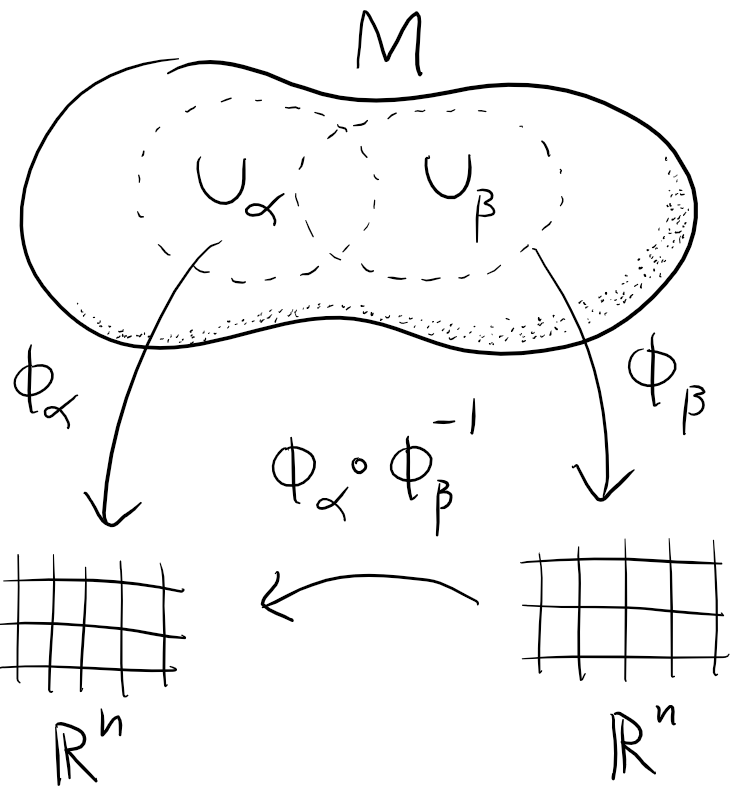
\includegraphics[width=0.35\textwidth]{img/manifold.png}
		\caption{The transition map between charts}
	\end{center}
\end{figure}
The crucial point is that the notion of differentiability from ordinary calculus applies since a transition map is a function from $\mathbb{R}^n$ to $\mathbb{R}^n$. $n$ is the \emph{dimension} of the manifold and we call $M$ an $n$-manifold for short. (We do not allow different connected components to have different dimensions.) So a differentiable manifold is in essence a space that locally looks Euclidean on which one can do calculus, but generally more than one chart is required to avoid coordinate singularities such as the poles on the Mercator projection map.

A \emph{Lie group} is a smooth manifold that has a compatible group structure i.e. group multiplication and inversion are smooth.\footnote{One can consider $C^k$ group manifolds for various $k$, but it turns out that every $C^0$ manifold with a compatible group structure can be made into a ($C^{\infty}$) Lie group in one and only one way (Hilbert's 5th problem). This is an even stronger statement than the fact from complex analysis that a complex $C^1$ function is automatically complex $C^{\infty}$.} A paradigmatic example of a Lie group is the general linear group $\gr{GL}{n,\mathbb{R}}$ of real invertible $n \times n$ matrices. It is an open subset (of $\mathbb{R}^{n^2}$) of matrices with non-zero determinant since the determinant is a polynomial and therefore continuous, and the image $\mathbb{R}\backslash \{0\}$ is open.\footnote{If $f$ is continuous, the pre-image $f^{-1}(X)$ of an open set $X$ is open.} Multiplication is linear and thus smooth, and inversion is smooth by Cramer's rule $A^{-1} = \text{adj}(A)/\det A$.

%Even thought a Lie group is topological in nature, all of its local features are captured by a single algebraic data, its Lie algebra. At each point $p$ on an $n$-manifold, $n$ orthogonal partial derivatives are linearly independent as vectors because when they act on any function $f$ on $M$,
%\begin{align}
%	(c_j \partial_j + c_k \partial_k )f = 0
%\end{align}
%if and only if $c_j=c_k=0$. Thus, they form an $n$-dimensional vector space $T_pM$ called the \emph{tangent space} at $p$. The \emph{Lie algebra} $\al{g}$ of a Lie group $G$ is the tangent space $T_eG$ at the identity together with a bilinear map $[\, , \, ]: \al{g} \times \al{g} \to \al{g}$, the \emph{Lie bracket}, which is antisymmetric $[x,y] = -[y,x]$ for any $x,y \in \al{g}$ (or equivalently $[x,x]=0$) and satisfies the Jacobi identity
%\begin{align}
%	[x,[y,z]] + [y,[x,z]] + [z,[x,y]] &= 0.
%\end{align}
%The last two properties

A Lie group $G$ may have an infinite number of generators, but it is a fact that any neighborhood of the identity element generates the component of $G$ connected to the identity. The idea of the Lie algebra is to describe $G$ by the ``linear approximation" of $G$ at the identity. Let $C^{\infty}(M)$ be the set of all smooth functions on $M$. Locally at each point $p$ on an $n$-manifold $M$, we can take partial derivatives in $n$ linearly independent directions. They are linearly independent as vectors because for every $f \in C^{\infty}(M)$ and $a \in \mathbb{R}$, if
\begin{align}
\sum_{j=1}^n a_j \partial_j f &= 0
\end{align}
then all $a_j=0$, thus they form an $n$-dimensional vector space called the \emph{tangent space} $T_p M$ at the point $p$. Globally, define a \emph{vector field} to be a linear function $X:C^{\infty}(M) \to C^{\infty}(M)$ obeying the Leibniz rule:
\begin{align}
X(fg) &= f X(g) + X(f) g
\end{align}
for every $f,g \in C^{\infty}(M)$ i.e. a \emph{derivation}. Intuitively, a vector field assigns to each point on a manifold a vector that allows us to take a derivative in that direction. Denote the set of all vector fields on $M$ by $\al{X}(M)$. Two vector fields can be composed together but the product is not a derivation. Instead $\al{X}$ can be endowed with the anticommutative product that gives another derivation, the \emph{Lie bracket}:\footnote{$C^{\infty}(M)$ is a commutative ring as functions can be multiplied together point-wise. So $\al{X}$ is a $C^{\infty}(M)$-module. The Lie bracket turns $\al{X}$ into a $C^{\infty}(M)$-algebra.}
\begin{align}
[X,Y] &= X \circ Y-Y \circ X.
\end{align}
The \emph{Jacobi identity}
\begin{align}
[X,[Y,Z]] + [Y,[Z,X]] + [Z,[X,Y]] &= 0,
\end{align}
says that the Lie bracket is a derivation with respect to itself
\begin{align}
	[X,[Y,Z]] &= [Y,[X,Z]] + [[X,Y],Z].
\end{align}
Given two smooth manifolds $M$ and $N$, and a smooth map $\varphi: M \to N$, we can construct a linear map from $\al{X}(M)$ to $\al{X}(N)$. The \emph{pushforward} $\varphi_*$ of $\varphi$ is defined to be
\begin{align}
[\varphi_*(X)](f) &\coloneqq  X[f \circ \varphi],
\end{align}
$X \in \al{X}(M)$ and $f \in C^{\infty}(N)$. When $M = G$ is a group, there is a distinct subset of vector fields whose value everywhere can be translated from the value at the identity $e$ by the pushforward of (left) group multiplication $X(g) = g_* [X(e)]$. The \emph{Lie algebra} $\text{Lie}(G)$ of a $G$ is defined to be these \emph{left-invariant vector fields} isomorphic to $T_e G$.

From the discussion above, it will come as no surprise that an abstract \emph{Lie algebra} $\al{g}$ is defined as a vector space together with a bilinear map $[\, , \, ]: \al{g} \times \al{g} \to \al{g}$, which is antisymmetric $[X,Y] = -[Y,X]$ for any $X,Y \in \al{g}$ (or equivalently $[X,X]=0$) and satisfies the Jacobi identity
\begin{align}
[X,[Y,Z]] + [Y,[Z,X]] + [Z,[X,Y]] &= 0.
\end{align}

%------------------------------------
\subsection{Matrix Lie groups}\label{ch2:matrix-group}
%------------------------------------

There is more than one possible way to define a submanifold which, in turn, affects the definition of a Lie subgroup. A smooth map $\varphi:M \to N$ is an \emph{immersion} if its pushforward $\varphi_*$ has full rank $\dim M$ for every point $p$ on $M$. An \emph{immersed submanifold} $N \subset M$ is a subset of $M$ which is itself a smooth manifold and the inclusion map $\imath: N \xhookrightarrow[]{} M$ is an immersion. A stronger notion is that of an \emph{embedded submanifold}, an immersed submanifold such that the inclusion map is a homeomorphism. An embedded submanifold inherits the topological structure from the manifold while an immersed submanifold may not. An example of the latter is the ``figure 6" map that takes an open interval to a shape with a different topology \cite{FH}:

\begin{figure}[H]\label{fig:6}
	\begin{center}
		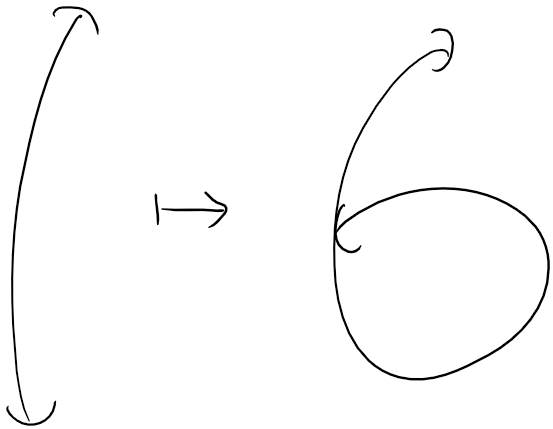
\includegraphics[width=0.35\textwidth]{img/figure-6-map.png}
		\caption{The ``figure 6" map}
	\end{center}
\end{figure}
\noindent 
Subgroups of a Lie group which are also immersed submanifolds are in one-one correspondence to Lie subalgebras of the group. Thus, one call these subgroups \emph{Lie subgroups}. Lie subgroups that are also embedded as submanifolds are not hard to come by as a result of the following theorem:
\begin{theorem}\label{thm:closed-subgroup} {\normalfont (The closed subgroup theorem) %\cite[Theorem 2.9, p.7]{Kirillov}
\cite[Theorem 20.12 p. 523]{Lee}}
	Any subgroup that is also a (topologically) closed subset \footnote{Technically, this theorem applies to discrete subgroups as any discrete group is a zero-dimensional Lie group, but we will not consider a discrete group in this context.} is a Lie subgroup which is embedded as a submanifold.
\end{theorem}
\noindent Note that the subset only needs to be closed in $G$ and not in any ambient space that $G$ is sitting in.

As an application of the theorem, since $\gr{GL}{n,\mathbb{R}}$ is a Lie group, a subgroup $G$ of $\gr{GL}{n,\mathbb{R}}$ such that any sequence of matrices in $G$ either converges in $G$ or outside $\gr{GL}{n,\mathbb{R}}$ (not invertible) is also a Lie group, called a \emph{(real) matrix Lie group}. The Lie algebra of a matrix group $G$ is the set of all matrices $X$ such that the exponential $e^X$ lands in $G$. For example the Lie algebra of $\gr{GL}{n,\mathbb{R}}$ is $\mat{n}{n}$, the set of all real $n \times n$ matrices. Let us give examples of real matrix groups that often appear in linear algebra, traditionally called the \emph{classical groups}, along with their Lie algebras, written in Fraktur.
\begin{enumerate}
	\item  The \emph{special linear group} is the connected component of matrices with determinant 1 in $\gr{GL}{n,\mathbb{R}}$.
	\begin{align}
	\gr{SL}{n,\mathbb{R}} &= \{ A \in \gr{GL}{n,\mathbb{R}} | \det A = 1 \} \\
	\al{sl}(n,\mathbb{R}) &= \{ X \in \mat{n}{n} | \Tr X = 0 \} \\
	\dim \gr{SL}{n,\mathbb{R}} &= n^2 - 1
	\end{align}
	
	\item The \emph{unitary group} is the group of matrices that preserve the Hermitian inner product $\braket{\, ,\,} :\mathbb{C}^{n} \times \mathbb{C}^{n} \to \mathbb{C}$:
	\begin{align}
		\braket{u,v} &= \sum_j u_j^* v_j.
	\end{align}
	The unitary Lie algebra is the set of all anti-Hermitian matrices.
	\begin{align}
	\gr{U}{n} &= \{ A \in \matc{n}{n} | A\dgg A = \id \} \\
	\al{u}(n) &= \{ X \in \matc{n}{n} | X\dgg  + X = 0 \} \\
	\dim \gr{U}{n} &= n^2
	\end{align}
	Despite the appearance of complex numbers, $\gr{U}{n}$ can be considered a real matrix group as $\mathbb{C}^n$ can be thought of as a real vector space $\mathbb{R}^{2n}$ of twice the dimensions.
	
	\item The \emph{special unitary group}.
	\begin{align}
	\gr{SU}{n} &= \{ A \in \gr{U}{n} | \det A = 1 \} \\
	\al{su}(n) &= \{ X \in \al{u}(n) | \Tr X = 0 \} \\
	\dim \gr{SU}{n} &= n^2 - 1
	\end{align}
	
	\item The \emph{(real) orthogonal group} $\gr{O}{n,\mathbb{R}}$ is the group of matrices that preserve the (symmetric) inner product $ g :\mathbb{R}^{n} \times \mathbb{R}^{n} \to \mathbb{R}$:
	\begin{align}
	g(u,v) &= \sum_{j=1}^{n} u_j v_j.
	\end{align}
	The connected component of matrices with determinant 1 constitutes the \emph{special orthogonal groups} $\gr{SO}{n,\mathbb{R}}$ which has the same Lie algebra, the set of all anti-symmetric matrices.
	\begin{align}
	\gr{O}{n,\mathbb{R}} &= \{ A \in \gr{GL}{n,\mathbb{R}} | A^T A = \id \} \\
	\gr{SO}{n,\mathbb{R}} &= \{ A \in \gr{O}{n,\mathbb{R}} | \det A = 1 \} \\
	\al{so}(n,\mathbb{R}) = \al{o}(n,\mathbb{R}) &= \{ X \in \mat{n}{n} | X^T + X = 0 \} \\
	\dim \gr{SO}{n,\mathbb{R}} &= \frac{n(n-1)}{2}
	\end{align}
	
	\item The (real) \emph{symplectic group} $\gr{Sp}{2n,\mathbb{R}}$ is the group of matrices that preserve the symplectic form $\omega :\mathbb{R}^{2n} \times \mathbb{R}^{2n} \to \mathbb{R}$:
	\begin{align}
	\omega(u,v) &= g(u,\Omega v) = \sum_{j=1}^{n} \left( u_j v_{n+j} - u_{n+j} v_j \right),
	\end{align}
	where
	\begin{align}
	\Omega &= \begin{pmatrix}
	{\huge 0} & \id \\
	-\id & {\huge 0}
	\end{pmatrix}.
	\end{align}
	\begin{align}
	\gr{Sp}{2n,\mathbb{R}} &= \{ A \in \gr{GL}{n,\mathbb{R}} | AJA^T = J \} \\
	\al{sp}(2n,\mathbb{R}) &= \{ A \in \mat{2n}{2n} | AJ + JA^T  = 0 \} \\
	\dim \gr{Sp}{2n,\mathbb{R}} &= n(2n+1)
	\end{align}
	A non-obvious fact, following from a Pfaffian identity \cite[p.119]{Procesi}, is that every symplectic matrix has determinant 1.
	
\end{enumerate}

$\gr{SO}{2n,\mathbb{R}}$ and $\gr{Sp}{2n,\mathbb{R}}$ are infinitesimally generated by $n$-mode quadratic fer\-mi\-on\-ic Hamiltonians and quadratic bosonic Hamiltonians, respectively.
The symmetric inner product and the symplectic form are, respectively, the real part and the imaginary part of the Hermitian inner product
\begin{align}
\braket{u,v} &= g(u,v) + i\omega(u,v).
\end{align}
(This is the local version of the K{\"a}hler structure (\autoref{app:kahler}).) Together with the fact that symplectic matrices have determinant 1, it follows that
\begin{align}\label{2-out-of-3-property}
\gr{U}{n} &\simeq \gr{SO}{2n,\mathbb{R}} \cap \gr{Sp}{2n,\mathbb{R}}.
\end{align}
This ortho-symplectic subgroup isomorphic to the unitary group is the group of particle-number-pre\-serv\-ing transformations for both bosons and fermions i.e. transformations that do not mix creation and annihilation operators.

%------------------------------------
\subsection{Representations of semisimple Lie algebras}\label{ch2:semisimple}
%------------------------------------

The theory is greatly simplified when we work over complex numbers. The \emph{complexification} $\al{g}^{\mathbb{C}} = \al{g} \oplus i\al{g}$ of a Lie algebra $\al{g}$ with the obvious Lie bracket is again a Lie algebra. An important example is $\al{gl}(n,\mathbb{C})$ which is the complexification of $\al{u}(n)$ because every complex matrix can be written as $A = B +iC$, where $B$ and $C$ are anti-Hermitian. Let us write for classical Lie algebras
\begin{align}
\al{sl}(n) &= \al{sl}(n,\mathbb{C}) = \al{u}(n)^{\mathbb{C}}, \\
\al{so}(n) &= \al{so}(n,\mathbb{C}) = \al{so}(n,\mathbb{R})^{\mathbb{C}}, \\
\al{sp}(n) &= \al{sp}(2n,\mathbb{C}) = \al{sp}(2n,\mathbb{R})^{\mathbb{C}}.
\end{align}

An \emph{ideal} $\al{k}$ of $\al{g}$ is a vector subspace
that absorbs every element of $\al{g}$ into itself: $[\al{k},\al{g}] \subset \al{k}$.
An ideal is a Lie subalgebra of $\al{g}$ and the Lie algebra of a normal subgroup of $G$. If $G$ has a nontrivial normal subgroup $K$, then to study $G$ we can study a simpler group $G/K$ through its Lie algebra $\al{g/k}$. A Lie algebra is \emph{simple} if it is not abelian (not every Lie bracket is zero) and has no nontrivial ideal. (The non-abelianity is there to make every simple Lie algebra semisimple, but it is a rather trivial condition to rule out $\al{u}(1)$, the only abelian Lie algebra which has no nontrivial ideal.) $\al{sl}(n)$ for $n \ge 2$, $\al{so}(n)$ for $n=3$ and $n \ge 5$, and $\al{sp}(n)$ are simple Lie algebras.

A \emph{representation} of a Lie algebra $\al{g}$ is a Lie algebra homomorphism $\pi: \al{g} \to \text{End}(V)$ i.e. a linear map respecting the Lie bracket:
\begin{align}
\pi([X,Y]) &= [\pi(X),\pi(Y)]
\end{align}
for all $X,Y \in \al{g}$. The \emph{adjoint representation} of $\al{g}$ is the Lie algebra homomorphism
\begin{align}
\text{ad}: \al{g} &\to \text{End}\al{g}, \\
\adrep X (Y) &= [X,Y].
\end{align}
It is the pushforward of the adjoint representation of its Lie group $G$ on the Lie algebra:
\begin{align}
\Adrep g (X) &= gXg^{-1}.
\end{align}
The two are related by the well known identity
\begin{align}
	e^Y X e^{-Y} &= e^{\adrep{Y}} X.
\end{align}
A bilinear form $\braket{\, , \,}$ is invariant with respect to the adjoint action if
\begin{align}
\braket{ \Adrep g (Y), \Adrep g (Z)} &= \braket{Y,Z}
\end{align}
or equivalently, by setting $g=e^{tX}$ and differentiating with respect to $t$
at the identity element,
\begin{align}
\braket{\adrep X (Y),Z} + \braket{Y,\adrep X (Z)} &= 0.
\end{align}
Any representation of a Lie algebra gives an invariant bilinear form $\braket{X,Y} =\\ \Tr [\pi(X) \pi(Y)]$. When $\pi$ is the adjoint representation, we have the \emph{Killing form}
\begin{align}\label{def:killing-form}
\kil{X}{Y} &\coloneqq \Tr (\adrep X \adrep Y),
\end{align}
which turns out to be proportional to $\Tr (XY)$ when the group is simple.
The Killing form of a compact real Lie group $G$ is negative semidefinite. To show this, we use the fact that every finite-dimensional representation of a compact group is unitary, thus every representation of $G$ sits inside $\al{u}(n) = \{ X \in \matc{n}{n} | X\dgg  + X = 0 \}$. Therefore, $\Tr (X^2) = - \Tr(XX\dgg ) = -\sum_{j,k} |X_{jk}|^2 \le 0$.

Over $\mathbb{C}$, a \emph{semisimple Lie algebra} $\al{g}$ can be defined by the following equivalent conditions: \cite[p.89]{Procesi}
\begin{enumerate}
	\item $\al{g}$ has no abelian ideal.
	\item  The Killing form on $\al{g}$ is non-degenerate. \emph{(Cartan's criteria for semisimplicity)}
	\item $\al{g} = \bigoplus_j \al{g}_j$ is a direct sum of simple Lie algebras $\al{g}_j$ mutually orthogonal with respect to the Killing form.
\end{enumerate}
A Lie group $G$ is simple or semisimple if its Lie algebra is simple or semisimple respectively. Given a complex Lie algebra $\al{g}$, there is a real Lie subalgebra $\al{k}$ whose complexification is $\al{g}$. If, moreover, $\al{g}$ is semisimple, then there is a compact, simply-connected group $K$ with $\al{k}^{\mathbb{C}} = \al{g}$, and representations of $\al{g}$, $\al{k}$, and $K$ can be studied interchangeably \cite[p.112]{Kirillov}.

The unique compact, simply-connected group associated with the classical group $\gr{SO}{n,\mathbb{R}}$ is its universal covering group, the \emph{spin group} $\gr{Spin}{n}$.\footnote{$\gr{SO}{n,\mathbb{R}}$ is not simply-connected. For instance, the rotation group $\gr{SO}{3,\mathbb{R}}$ is topologically a three-dimensional ball with antipodal points identified: the two angles parametrize the axis of rotation and the radius parametrizes the angle of rotation. Antipodal points are $\pi$ and $-\pi$ rotations. Any nontrivial path between antipodal points is a loop that cannot be shrunk to a single point.}
That is, $\gr{Spin}{n}$ is a unique compact, simply-connected Lie group such that there exists a surjective (onto) Lie group homomorphism
\begin{align}\label{def:spin-group}
	\gr{Spin}{n} \twoheadrightarrow \gr{SO}{n,\mathbb{R}}.
\end{align}
It is also a double cover of $\gr{SO}{n,\mathbb{R}}$, meaning that there is a representation of $\gr{Spin}{n}$ which is a representation of $\gr{SO}{n,\mathbb{R}}$ only up to a sign (projective representation), called a \emph{spinor representation}.

%------------------------------------
\subsection{Roots and weights}\label{ch2:root}
%------------------------------------

The structure theory of complex semisimple Lie algebras mimics and generalizes the $\al{su}(2)$ case familiar to every physicist from the quantum theory of angular momentum, which we briefly remind the reader here. Consider the Pauli matrices:
\begin{align}
X & =\left(\begin{array}{cc}
0 & 1\\
1 & 0
\end{array}\right),&
Y & =\left(\begin{array}{cc}
0 & -i\\
i & 0
\end{array}\right),&
Z & =\left(\begin{array}{cc}
1 & 0\\
0 & -1
\end{array}\right).
\end{align}
$\al{su}(2)$ is a real Lie algebra whose basis can be chosen to be $\{ iX,iY,iZ \}$,
\begin{align}
[iX,iY] &= -2iZ,&
[iY,iZ] &= -2iX,&
[iZ,iX] &= -2iY.
\end{align}
Physicists' version of the commutation relations of $\al{su}(2)$ are in fact those of $\al{sl}(2) = \al{su}(2)^{\mathbb{C}}$:
\begin{align}
[X,Y] & =2iZ,&
[Y,Z] & =2iX,&
[Z,X] & =2iY,
\end{align}
In the basis
\begin{align}
H & =Z,&
E_{\pm} & =\frac{X \pm iY}{2}
\end{align}
one has the commutation relations
\begin{align}
[H,E_{\pm}] &= \pm 2E_{\pm},&
[E_+,E_-] & =H.
\end{align}
From this, one derives that there is exactly one distinct irrep in each dimension $\lambda+1$---referred to in the physics jargon as the spin-$\lambda/2$ representation---and these are all the finite-dimensional irreps of $\gr{sl}{2}$. Each irrep $(\pi_{\lambda},V_{\lambda})$ decomposes into mutually orthogonal eigenvectors of $\pi_j(H)$.
\begin{align}
\pi_{\lambda}(H) \ket{\lambda,\mu} &= \mu \ket{\lambda,\mu}.
\end{align}
The integral eigenvalues $\mu$ are \emph{weights} and the eigenvectors are \emph{weight vectors}. $V_{\lambda}$ can be constructed by recursively applying the lowering operator $E_-$ starting from the highest weight vector:
\begin{align}
\pi_{\lambda}(E_+) \ket{\lambda,\lambda} &= 0,
\end{align}
making use of the relation
\begin{align}
\pi_{\lambda}(H) \pi_{\lambda}(E_-) \ket{\lambda,\mu} &= (\mu - 2)\pi_{\lambda}(E_-) \ket{\lambda,\mu} %\\
%\pi_{\lambda}(H) \pi_{\lambda}(F) \ket{\lambda,\mu} &= (\lambda - 2)\pi_{\lambda}(F) \ket{\lambda,\mu}.
\end{align}

For general complex semisimple Lie algebras, $H$ generalizes to a \emph{Cartan subalgebra}, a maximal abelian subalgebra $\al{h} \subset \al{g}$ such that $\adrep H$ is diagonalizable for every $H \in \al{h}$ \cite[Proposition 2.13, p.136]{Knapp}. (Beware that this definition is only valid for semisimple Lie algebras.)
Every complex semisimple Lie algebra of $G$ has a Cartan subalgebra, and a Cartan subalgebra is the complexified Lie algebra of some maximal torus in $G$. A Cartan subalgebra is not unique, but all Cartan subalgebras are conjugated, thus have the same dimension called the \emph{rank} of the Lie algebra.

The most important result about semisimple Lie algebras---much more important than the definition of semisimple Lie algebras itself \cite{Kirillov}---is the \emph{root space decomposition} of the adjoint representation $\al{g}$. Since $\al{h}$ is abelian, all $\adrep H$ are simultaneously diagonalizable, decomposing $\al{g}$ into a direct sum
\begin{align}
\al{g} &\stackrel{\al{g}}{\simeq} \al{h} \oplus \bigoplus_{\alpha \in \mathcal{R}}\al{g}_{\alpha},
\end{align}
where
\begin{align}
	 \al{g}_{\alpha} &= \{ E_{\alpha} \mid [H,E_{\alpha}] = \alpha(H) E_{\alpha}, \forall H \in \al{h} \}
\end{align}
is called a \emph{root space}. Each \emph{root} $\alpha \in \al{h}^* - \{0\}$ (linear non-zero forms on $\al{h}$) corresponds to an eigenvalue $\alpha(H)$ and a \emph{root vector} $E_{\alpha}$. The finite set $\mathcal{R}$ of roots is called the \emph{root system}. Roots are special cases of weights in the adjoint representation. Roots and root spaces have the following properties:
\begin{enumerate}
	
	\item Every $\al{g}_{\alpha}$ is one-dimensional.
	
	\item\label{root-space-orthogonality} Writing $\al{g}_0 = \al{h}$, taking a commutator is equivalent to adding roots:
	\begin{align}
	[\al{g}_{\alpha} , \al{g}_{\beta}] \subset \al{g}_{\alpha+\beta}.
	\end{align}
	Furthermore, $\al{g}_{\alpha}$ and $\al{g}_{\beta}$ are orthogonal with respect to the Killing form whenever $\alpha + \beta \neq 0$ (whereas $\al{g}_{\alpha}$ and $\al{g}_{-\alpha}$ are never orthogonal).
	
	\item\label{root-span} $\mathcal{R}$ spans $\al{h}^*$.
	
	\item\label{positive-root} For every $\alpha \in \mathcal{R}$, the only non-zero multiples of $\alpha$ that are in $\mathcal{R}$ are $\pm \alpha$.
	
\end{enumerate}
%To prove \ref{root-space-orthogonality}, note that
%\begin{align}
%	(\adrep E_{\alpha} \adrep E_{\beta}) E_{\gamma} &= E_{(\alpha + \beta) + \gamma}.
%\end{align}
%$\adrep E_{\alpha} \adrep E_{\beta}$
%therefore has no diagonal element, making the Killing form vanishes.
A consequence of property \ref{root-space-orthogonality} is that the Killing form restricted to $\al{h}$ is non-degenerate and thus can be used to identify $\al{h}$ and $\al{h}^*$. Even though there is \emph{a priori} no preferred basis for $\al{h}$, there is a preferred basis in $\al{h}^*$ consisting of the roots. In particular, the Killing form associates to each $\alpha \in \al{h}^*$ %and $E_{\alpha} \in \al{g}_{\alpha}$
, $H_{\alpha} \in \al{h}$ via
\begin{align}
\kil{H_{\alpha}}{H} &= \alpha(H).
\end{align}
To keep the notation tidy, we write the inner product of two roots as
\begin{align}
\braket{\alpha,\beta} &\coloneqq \kil{H_{\alpha}}{H_{\beta}} = \alpha(H_{\beta}) = \beta(H_{\alpha}).
\end{align}
The number $\braket{\alpha,\alpha}$ is called the \emph{length} of the root $\alpha$. The \emph{Cartan basis} is
\begin{align}
[H,E_{\alpha}] &= \alpha(H) E_{\alpha}, \\
[E_{\alpha}, E_{\beta}] &=
\begin{cases}
N_{\alpha \beta} E_{\alpha + \beta}, & \alpha + \beta \neq 0, \alpha + \beta \in \mathcal{R}, \\
\braket{\alpha,-\alpha} H_{\alpha}, & \alpha + \beta = 0,
\end{cases}
\end{align}
where the last commutator follows directly from the invariance of the Killing form $\kil{[E_{\alpha}, E_{-\alpha}]}{H} = \kil{E_{\alpha}}{[E_{-\alpha}, H]}$ and $[H,[E_{\alpha},E_{-\alpha}]]=0$.

Simple roots are introduced to provide a succinct description of complex semisimple Lie algebras. From properties \ref{root-span} and \ref{positive-root} of a root system, if we make an arbitrary choice of which of the roots $\pm \alpha$ to call \emph{positive}, then the set of positive roots $\mathcal{R}_+$ spans $\al{h}^*$. The collection $\Delta$ of \emph{positive simple roots}, positive roots that cannot be written as nontrivial linear combinations of other roots, forms a basis for $\al{h}^*$.\footnote{Each positive simple root corresponds to a copy of $\al{sl}(2)$. To see this, rescale $E_{\alpha}$ and $E_{-\alpha}$ so that $\kil{E'_{\alpha}}{E'_{-\alpha}} = 2/\braket{\alpha,\alpha}$ and set $H'_{\alpha} = 2H_{\alpha}/\braket{\alpha,\alpha}$. Then
	\begin{align}
	[H',E'_{\pm}] &= \pm 2E'_{\pm},&
	[E'_+,E'_-] &= H',
	\end{align}
	is the basis of a subalgebra isomorphic to $\al{sl}(2)$.}  The \emph{Cartan matrix} is defined to be the matrix of integers
\begin{align}
A_{jk} &\coloneqq \frac{2\braket{\alpha_k,\alpha_j}}{\braket{\alpha_j,\alpha_j}}.
\end{align}
The Cartan matrix depends on the choice of positive simple roots $\Delta$ but different choices give Cartan matrices that are conjugate to each other by a permutation matrix. A unique \emph{Dynkin diagram} can be associated with equivalent Cartan matrices by the following algorithm:
\begin{enumerate}
	\item Draw a vertex for each simple root $\alpha_j$.
	\item Connect vertices $\alpha_j$ and $\alpha_k$ by $A_{jk}A_{kj}$ edges.
	\item Draw an arrow pointing from a longer root to a shorter root. (The arrow's head is the greater-than sign $>$.)
\end{enumerate}
The classical Lie algebras introduced earlier are all simple. In fact, they exhaust the list of infinite families of finite-dimensional, complex semisimple Lie algebras parametrized by the number of positive roots $n$, which is also the same as the rank. Belows are the Dynkin diagrams, built from right to left, of the classical groups.
\begin{center}
	\begin{tikzpicture}
	
	\draw (0,0) -- (1,0);
	\draw (2,0) -- (2.7,0);
	\draw (1,0) -- (2,0);
	\draw (3.3, 0) -- (4,0);
	\draw (4,0) -- (5,0);
	
	\draw[fill=white] (0,0) circle(.1);
	\draw[fill=white] (1,0) circle(.1);
	\draw[fill=white] (2,0) circle(.1);
	\draw[fill=white] (4,0) circle(.1);
	\draw[fill=white] (5,0) circle(.1);
	
	\node at (3,0) {$\cdots$};
	\node at (-2.15,0) {$A_n = \al{sl}(n+1)$};
	
	\end{tikzpicture}
	
	\begin{tikzpicture}
	
	\draw (0,0) -- (2.7,0);
	\draw (3.3, 0) -- (4,0);
	\draw (4,0.1) -- (5,0.1);
	\draw (4,-0.1) -- (5,-0.1);
	\draw (4.4,0.2) -- (4.6,0);
	\draw (4.4,-0.2) -- (4.6,0);
	
	\draw[fill=white] (0,0) circle(.1);
	\draw[fill=white] (1,0) circle(.1);
	\draw[fill=white] (2,0) circle(.1);
	\draw[fill=white] (4,0) circle(.1);
	\draw[fill=white] (5,0) circle(.1);
	
	\node at (3,0) {$\cdots$};
	\node at (-2,0) {$B_n = \al{so}(2n+1)$};
	
	\end{tikzpicture}
	
	\begin{tikzpicture}
	
	\draw (0,0) -- (2.7,0);
	\draw (3.3, 0) -- (4,0);
	\draw (4,0.1) -- (5,0.1);
	\draw (4,-0.1) -- (5,-0.1);
	\draw (4.4,0) -- (4.6,0.2);
	\draw (4.4,0) -- (4.6,-0.2);
	
	\draw[fill=white] (0,0) circle(.1);
	\draw[fill=white] (1,0) circle(.1);
	\draw[fill=white] (2,0) circle(.1);
	\draw[fill=white] (4,0) circle(.1);
	\draw[fill=white] (5,0) circle(.1);
	
	\node at (3,0) {$\cdots$};
	\node at (-2.45,0) {$C_n = \al{sp}(n)$};
	
	\end{tikzpicture}
	
	\begin{tikzpicture}
	
	\draw (0,0) -- (2.7,0);
	\draw (3.3, 0) -- (4,0);
	\draw (4,0) -- (5,-.5);
	\draw (4,0) -- (5,.5);
	
	\draw[fill=white] (0,0) circle(.1);
	\draw[fill=white] (1,0) circle(.1);
	\draw[fill=white] (2,0) circle(.1);
	\draw[fill=white] (4,0) circle(.1);
	\draw[fill=white] (5,-.5) circle(.1);
	\draw[fill=white] (5,.5) circle(.1);
	
	\node at (3,0) {$\cdots$};
	\node at (-2.35,0) {$D_n = \al{so}(2n)$};
	
	\end{tikzpicture}
\end{center}


\noindent That is, $ \ran \al{sl}(n) = n-1$, $\ran \al{so}(n) = \lfloor n/2 \rfloor$, and $\ran \al{sp}(n) = n$. We also notice from the diagrams isomorphisms of low-dimensional Lie algebras: $\al{su}(2) \allowbreak = \al{so}(3) = \al{sp}(1)$, $\al{so}(4) = \al{sl}(2) \oplus \al{sl}(2)$, $\al{so}(5) = \al{sp}(2)$, and $\al{su}(4) = \al{so}(6)$. ($\al{u}(1) = \al{so}(2)$ are abelian, thus not simple.)

Every representation of a complex semisimple Lie algebra can be characterized by its highest weight. In a representation $(\pi,V)$, a simultaneous eigenvector of the restriction of $\pi$ to the Cartan subalgebra $\ket{v} \in V$ is called a vector of \emph{weight} $\lambda$ if
\begin{align}
\pi(H) \ket{v} = \lambda(H) \ket{v}.
\end{align}
$V$ decomposes into (not necessarily one-dimensional) \emph{weight spaces}:
\begin{align}
V &\stackrel{\al{g}}{\simeq}  \bigoplus_{\lambda}V_{\lambda},
\end{align}
where
\begin{align}
	V_{\lambda}
	&\coloneqq \bigoplus_{\lambda} \{ \ket{v} \in V \big| \pi(H) \ket{v} = \lambda(H) \ket{v}, \forall H \in \al{h} \}.
\end{align}
The weights can be given a partial ordering: $\lambda \succeq \mu$ if and only if the difference $\lambda - \mu$ is a positive linear combination of positive simple roots. A weight then is a \emph{highest weight} of $\pi$ if $\lambda \succ \mu$ for every weight $\mu$ of $\pi$. A weight $\lambda$ is said to be \emph{integral} if $2\braket{\lambda,\alpha}/\braket{\alpha,\alpha}$ is an integer for every positive simple root $\alpha \in \Delta$. If the integer is in addition positive, the weight is said to be \emph{dominant integral}. It turns out that every weight is integral. The \emph{highest weight theorem} guarantees that each and every dominant integral weight $\lambda$ gives distinct finite dimensional irreps of $\al{g}$ with the highest weight $\lambda$ and every finite dimensional irrep of $\al{g}$ arises in this way. One then applies negative simple roots to the highest weight vector to generate an orthonormal basis for each irrep.

%------------------------------------
\subsection{Realizations of classical Lie algebras by creation and annihilation operators}\label{ch2:physics-realization}
%------------------------------------

$\al{gl}(n)$ can be explicitly realized by operators quadratic and linear in either the bosonic or fermionic creation and annihilation operators \cite[Chapter 9 and 10]{iachello}. Since matrix Lie algebras are Lie subalgebras of $\al{gl}(n)$, all matrix Lie algebras have bosonic and fermionic realizations. (The bosonic realizations of the classical Lie algebras are summarized in \cite[\S 10.4, p. 309]{Barut}. Well known is the bosonic realization of $\al{gl}(n)$ called the Schwinger representation \cite{Schwinger}.) To prove the realizations, we only need to verify that the appropriate bosonic or fermionic operators are eigenvectors of the adjoint representation of a Cartan subalgebra with the eigenvalues as the roots. The roots of the classical Lie algebras can be found on a case-by-case basis \cite{FH}.

The fermionic creation and annihilation operators for $n$ modes are defined by the canonical anticommutation relation
\begin{align}
\{a_j,a_k\dgg \} &= \delta_{jk}\id, &
\{a_j,a_k\}&=0.
\end{align}
To simplify the notations, let us define
\begin{align}
E^j{}_k &\coloneqq a_j\dgg a_k - \frac{1}{2}\delta_{jk}\id, &
E^{jk} 	&\coloneqq a_j\dgg a_k\dgg, &
E_{jk} &\coloneqq a_j a_k.
\end{align}
Then
\begin{align}
	E^j{}_k{}\dgg &= E^k{}_j, &
	E^{jk \dagger} &= E_{kj}, &
	E_{jk} &= -E_{kj},
\end{align}
and
\begin{equation*}
	\noindent\begin{minipage}[t]{.5\textwidth}
		\begin{align}
		[a_j,a_k] &= 2E_{jk}, \\
		[a_j\dgg,a_k] &= 2E^j{}_k, \\
		[a_j,E^k{}_l] &= \delta_{jk} a_l, \label{so(2n+1)-commutation-relations} \\
		[a_j,E^{kl}] &= \delta_{jk} a_l\dgg - \delta_{jl}a_k\dgg, \\
		[a_j,E_{kl}] &= 0,
		\end{align}
	\end{minipage}%
	\begin{minipage}[t]{.5\textwidth}
		\begin{align}
		[E^j{}_k,E^l{}_m] &= \delta_{lk}E^j{}_m - \delta_{jm}E^l{}_k, \label{u(n)-commutation-relations} \\
		[E^j{}_k,E_{lm}] &= \delta_{jm}E_{kl} - \delta_{jl}E_{km}, \\
		\begin{split}
			[E^{jk},E_{lm}] &= \delta_{jm}E^k{}_l + \delta_{kl}E^j{}_m \\
			&- \delta_{jl}E^k{}_m - \delta_{km}E^j{}_l,
		\end{split} \\
		[E_{jk},E_{lm}] &= 0,
		\end{align}
	\end{minipage} \nonumber
\end{equation*}

Now we are ready to give the fermionic realizations of the orthogonal Lie algebras and of $\al{gl}(n)$, which for our purpose, is thought of as a subalgebra of the orthogonal ones.

%------------------------------------
\subsubsection{$\text{B}_n = \al{so}(2n+1)$}
%------------------------------------
$\al{so}(2n+1)$ can be realized by all quadratic and linear fermionic operators.
The $n$-dimensional Cartan subalgebra $\al{h}$ can be chosen to be the span of $\{E^j{}_j\}$.
Let $e_j$ be a linear form such that $e_j (E^k{}_k) = \delta_{jk}$. The roots are
\begin{align}
	R &= \{ e_j \pm e_k, -(e_j \pm e_k), \pm e_j |j \neq k \}.
\end{align}
Positive simple roots can be chosen to be
\begin{align}
	\Delta &= \{ -e_1, e_1 - e_2, \dots, e_{n-1} - e_n \}.
\end{align}
Using the commutation relations eq. \eqref{so(2n+1)-commutation-relations} and eq. \eqref{u(n)-commutation-relations},
\begin{align}
[E^j{}_j, a_k] &= -[a_k, E^j{_j}]\dgg = -\delta_{jk} a_k = -e_k(E^j{}_j) a_k, \\
[E^j{}_j, E^k{}_l] &= \delta_{jk} E^j{}_l - \delta_{jl} E^k{}_j = (e_k - e_l) (E^j{}_j) E^k{}_l.
\end{align}
Therefore, we have
\begin{align}
	\Delta = \{ a_1, a_1\dgg a_2, \dots, a_{n-1}\dgg a_n \}.
\end{align}
Via the Killing form, the root $-e_j$ is associated, up to a scalar multiple, with $H_{\alpha_j} = -E^j{}_j$. Similarly, the roots $\alpha_j = e_{j-1} - e_j$ are associated with $H_{\alpha_j} = E^{j-1}{}_{j-1} - E^j{}_j$, up to the same scalar multiple. One can then calculate the inner product $\braket{\alpha_j,\alpha_k} = \kil{H_{\alpha_j}}{H_{\alpha_k}}$ between all pair of roots to obtain the Dynkin diagram:
\begin{center}
	\begin{tikzpicture}
	
	\draw (0.5,0.1) -- (1.5,0.1);
	\draw (0.5,-0.1) -- (1.5,-0.1);
	\draw (0.9,0) -- (1.1,0.2);
	\draw (0.9,0) -- (1.1,-0.2);
	\draw (2.5,0) -- (3.1,0);
	\draw (3.8,0) -- (4.7,0);
	\draw (5.3,0) -- (6,0);
	
	\draw[fill=white] (0,0) circle(.5);
	\draw[fill=white] (2,0) circle(.5);
	\draw[fill=white] (3.5,0) circle(.5);
	\draw[fill=white] (6.5,0) circle(.5);
	
	\node at (5.05,0) {$\cdots$};
	\node at (0,0) {$a_1$};
	\node at (2,0) {$a\dgg_1 a_2$};
	\node at (3.5,0) {$a\dgg_2 a_3$};
	\node at (6.5,0) {\scriptsize $a_{\!n\!-\!1}\!\dgg a_n$};
	\end{tikzpicture}
\end{center}

%------------------------------------
\subsubsection{$\text{D}_n = \al{so}(2n)$}
%------------------------------------

$\al{so}(2n)$ is a subalgebra of $\al{so}(2n+1)$ consisting of all quadratic fermionic operators. The Cartan subalgebra remains the same as $\al{so}(2n+1)$ (though $H_{\alpha_j}$ changes depending on the roots). We no longer have the linear term, so the roots and positive simple roots are
\begin{align}
R &= \{ e_j \pm e_k, -(e_j \pm e_k) |j \neq k \}, \\
\Delta &= \{-(e_1 + e_2), e_1 - e_2, \dots, e_{n-1} - e_n \},
\end{align}
Since
\begin{align}
	[E^j{}_j, E_{kl}] &= \delta_{jl} E_{jk} - \delta_{jk} E_{jl}
	= - \delta_{jl} E_{kl} - \delta_{jk} E_{kl}  \nonumber \\
	&= -(e_k + e_l) (E^j{}_j) E_{kl},
\end{align}
the positive simple roots are
\begin{align}
\Delta &= \{a_1a_2, a_1\dgg a_2, \dots, a_{n-1}\dgg a_n \},
\end{align}
and the Dynkin diagram is
\begin{center}
	\begin{tikzpicture}
	
	\draw (0.3,-1) -- (1,-0.3);
	\draw (0.3,1) -- (1,0.3);
	\draw (1,0) -- (2.7,0);
	\draw (3,0) -- (4,0);
	\draw (4.6,0) -- (5.5,0);
	
	\draw[fill=white] (0,-1.3) circle(.5);
	\draw[fill=white] (0,1.3) circle(.5);
	\draw[fill=white] (1.3,0) circle(.5);
	\draw[fill=white] (2.8,0) circle(.5);
	\draw[fill=white] (5.8,0) circle(.5);
	
	\node at (4.35,0) {$\cdots$};
	\node at (0,-1.3) {$a\dgg_1 a_2$};
	\node at (0,1.3) {$a_1 a_2$};
	\node at (1.3,0) {$a\dgg_2 a_3$};
	\node at (2.8,0) {$a\dgg_3 a_4$};
	\node at (5.8,0) {\scriptsize $a\dgg_{\!n\!-\!1}\! a_n$};
	\end{tikzpicture}
\end{center}

%------------------------------------
\subsubsection{$\text{A}_n = \al{sl}(n+1)$}
%------------------------------------

By eq. \eqref{u(n)-commutation-relations}, $\{ E^j{}_k \}$ is a subalgebra of $\al{so}(2n)$ having the root structure isomorphic to that of $\al{gl}(n) = \al{sl}(n) \oplus \al{u}(1)$, where the $\al{u}(1)$ is the total number operator $\sum_j E^j{}_j$. Consider only the simple part $\al{sl}(n)$. The Cartan subalgebra remains the same as that of the orthogonal Lie algebras. The roots and positive simple roots are
\begin{align}
	R &= \{ e_j - e_k |j \neq k \}, \\
	\Delta &= \{ e_j - e_k |j < k \}.
\end{align}
The ``two-mode squeezing" $a_j a_k$ is removed from the roots:
\begin{align}
	\Delta &= \{ a_1\dgg a_2, \dots, a_{n-1}\dgg a_n \}
\end{align}
\begin{center}
	\begin{tikzpicture}
	
	\draw (0,0) -- (2.7,0);
	\draw (3.3, 0) -- (4,0);
	
	\draw[fill=white] (0,0) circle(.5);
	\draw[fill=white] (1.5,0) circle(.5);
	\draw[fill=white] (4.5,0) circle(.5);
	
	\node at (3,0) {$\cdots$};
	\node at (0,0) {$a\dgg_1 a_2$};
	\node at (1.5,0) {$a\dgg_2 a_3$};
	\node at (4.5,0) {\scriptsize $a\dgg_{\!n\!-\!1}\! a_n$};
	\end{tikzpicture}
\end{center}

%------------------------------------
\subsubsection{$\text{C}_n = \al{sp}(n)$}
%------------------------------------

We do not use the root system of the symplectic Lie algebra anywhere in this dissertation, but note that the bosonic realization
\begin{align}
	[b_j,b_k\dgg] &= \delta_{jk}\id.
\end{align}
of positive simple roots of $\al{sp}(n)$:
\begin{align}
	\Delta &= \{-2e_1, e_1 - e_2, \dots, e_{n-1} - e_n \} \\
	&= \Bigl\{ \frac{b_1^2}{2} ,b_1\dgg b_2, \dots, b_{n-1}\dgg b_n \Bigr\}
\end{align}
	\begin{center}
		\begin{tikzpicture}
		
		\draw (0.5,0.1) -- (1.5,0.1);
		\draw (0.5,-0.1) -- (1.5,-0.1);
		\draw (1.1,0) -- (0.9,0.2);
		\draw (1.1,0) -- (0.9,-0.2);
		\draw (2.5,0) -- (3.1,0);
		\draw (3.8,0) -- (4.7,0);
		\draw (5.3,0) -- (6,0);
		
		\draw[fill=white] (0,0) circle(.5);
		\draw[fill=white] (2,0) circle(.5);
		\draw[fill=white] (3.5,0) circle(.5);
		\draw[fill=white] (6.5,0) circle(.5);
		
		\node at (5.05,0) {$\cdots$};
		\node at (0,0) {\large $\frac{b_1^2}{2}$};
		\node at (2,0) {$b\dgg_1 b_2$};
		\node at (3.5,0) {$b\dgg_2 b_3$};
		\node at (6.5,0) {\scriptsize $b_{\!n\!-\!1}\!\dgg b_n$};
		\end{tikzpicture}
	\end{center}
look very similar to those of $\al{so}(2n+1)$ except that the two-mode squeezing is replaced by a single-mode squeezing.

%------------------------------------
\section{Harmonic analysis on multiplicity-free spaces}\label{ch2:gelfand}
%------------------------------------

Traditional Fourier analysis on the real line $\mathbb{R}$ or the circle $U(1)$ is the multiplicity-free decomposition of the regular representation of an abelian group. A simple characterization of the multiplicity-free property for the representation $L^2(G/K)$ of a homogeneous space $G/K$ can be given in terms of Frobenius reciprocity. Since $L^2(G/K)$ is the representation $\ind{\mathbb{C}}{K}{G}$ induced from the trivial representation, $L^2(G/K)$ is multiplicity-free if and only if the trivial irrep of $K$ appears at most once in any irrep $V_{\lambda}$,
\begin{align}
\dim \text{Hom}_G ( V_{\lambda}, L^2(G/K) ) = \dim \text{Hom}_K (\text{Res} V_{\lambda}, \mathbb{C}) \le 1.
\end{align}

Gelfand found that $L^2(G/K)$ is multiplicity-free if and only if the space of $K$-bi-invariant functions $L^1(K\backslash G/K)$ is commutative with respect to convolution product \cite{gelfand1950spherical}.\footnote{$L^1(K\backslash G/K)$ turns out to be the space of intertwiners $\text{End}_G(L^2(G/K))$, the analogue of the \emph{Hecke algebra} for finite groups.} Such a pair $(G,K)$ is called a \emph{Gelfand pair}. We will also call the coset space $G/K$ a \emph{multiplicity-free space} if $(G,K)$ is a Gelfand pair.
%\footnote{Multiplicity-free spaces are also called \emph{commutative spaces} because of Gelfand's criterion \cite{wolf2007harmonic}, but we will not use that term since it can be confused with the term (non-)commutative \emph{phase} space.} 
The notion of a \emph{(zonal) spherical function} of an irrep $(\rep_{\lambda},V)$ makes sense on a multiplicity-free space $G/K$. It is the matrix element of $\rep_{\lambda}$ of the $K$-invariant vector in $V$, the unique trivial irrep of $K$ appearing in $V$, and they form an orthogonal basis for $L^1(K\backslash G/K)$ \cite[\S 17.3]{Vilenkin3}.

%------------------------------------
\subsection{Symmetric spaces and $KAK$ decomposition}\label{ch2:kak}
%------------------------------------

Most relevant to us is the fact that fermionic phase spaces $\homsp{SO}{2n}{U}{n}$ and $\homsp{SO}{2n+1}{U}{n}$ are multiplicity-free \cite[and references therein]{wolf2007harmonic}, and in principle, the $K$-invariant vectors are the only thing we need to construct their corresponding quasi-probability representations (\autoref{ch3:construction}). Especially, $\homsp{SO}{2n}{U}{n}$ has a special symmetry property that implies the multiplicity-free property. Let $G$ be a Lie group with a Lie algebra $\al{g}$. A nontrivial involutive Lie algebra automorphism (homomorphism onto itself) $\theta$,
\begin{align}
\theta^2 &= \id,
\end{align}
called a \emph{Cartan involution} is diagonalizable and splits $\al{g}$ into the $+1$ and $-1$ ei\-gen\-spaces $\al{k}$ and $\al{p}$ respectively. Equivalently, these subspaces obey the defining commutation relations 
\begin{align}
[\al{k},\al{k}] &\subset \al{k}, \\
[\al{k},\al{p}] &\subset \al{p}, \label{reductive} \\
[\al{p},\al{p}] &\subset \al{k}. \label{symmetric}
\end{align}
Such a pair $(G,K)$ is called a \emph{symmetric pair}, and $G/K$ is called a \emph{symmetric space} \cite{Helgason}.
We directly see from the fermionic commutation relations that $\homsp{SO}{2n}{U}{n}$ is a symmetric space while $\homsp{SO}{2n+1}{U}{n}$ is not. The multiplicity-free property can be proved directly from the existence of an involution using the Gelfand's criterion \cite[pp.36-37]{Gangolli} or from the $KAK$ decomposition below.

For $G$ non-compact semisimple, the Cartan involution leads to the \emph{Cartan decomposition}, which is a generalization of the polar decomposition for invertible matrices when $G/K = \homsp{GL}{n,\mathbb{R}}{O}{n,\mathbb{R}}$. It can be proved that the bilinear form defined by the involution
\begin{align}
	\kil{X}{\theta Y}
\end{align}
is negative definite \cite{Knapp}. Thus the Killing form is negative definite on $K$ and positive definite on $P$, showing that $K$ is a maximal compact subgroup of $G$. $G$ has the Cartan decomposition at the Lie algebra level $\al{g} = \al{k} \oplus \al{p}$ and at the Lie group level $G = KP = PK$ where $P = \exp \al{p}$. But for $G$ compact, the only Cartan involution is the trivial one $\theta= \id$ because a maximal compact subgroup of a compact group $G$ is $G$ itself. Nevertheless, a similar decomposition also works in the setting when $G$ is compact semisimple. Let $\al{g}$ now be a real non-compact semisimple Lie algebra and consider its complexification $\al{g}^{\mathbb{C}}$. Corresponding to the Cartan decomposition $\al{g} = \al{k} \oplus \al{p}$ is the dual compact Lie algebra $\tilde{\al{g}} = \al{k} \oplus i\al{p}$ with the decomposition $\widetilde{G} = KP = PK $. The decomposition is unique as long as $g \in G$ is full rank. \cite[\S 1.2.3, p.56]{Vilenkin1}

The \emph{$KAK$ decomposition} follows from the polar decomposition and the fact that the adjoint action of $K$ generates the entire $P$ from any maximal abelian subgroup $A \in P$ with Lie algebra $\al{a}$.
\begin{align}\label{KAK}
\al{g} &= \al{k} \oplus \bigcup_{k \in \al{k}} [k,\al{a}], \\
G &= K \left( \bigcup_{k \in K} kAk^{-1} \right) = KAK.
\end{align}
The dimension of the maximal abelian subgroup is also called the \emph{rank} of the symmetric space, which is well known for irreducible symmetric spaces \cite{Helgason}. $K$-bi-invariant functions are precisely functions on a maximal abelian subgroup $A$ in $KAK$. Therefore, symmetric spaces are multiplicity-free by Gelfand's criterion and every $K$-bi-invariant function is a linear combination of the zonal spherical functions.

%------------------------------------
\subsection{Spherical functions}\label{ch2:spherical}
%------------------------------------

Recall from the Peter-Weyl theorem (Theorem \ref{thm:peter-weyl}) that the matrix elements $\{ \sqrt{d_{\lambda}} \\ \rep_{\lambda}(g)_{jk} \}$ form an orthonormal basis of $L^2(G)$ for a compact group $G$. Functions on $G/K$ are precisely functions on $G$ that are right $K$-invariant, so they must be spanned by the
\begin{align}
\sqrt{d_{\lambda}} \rep_{\lambda}(g)_{\mu 0} = \sqrt{d_{\lambda}} \braket{\lambda m|\rep_{\lambda}(g)|\lambda 0},
\end{align}
They obey two important identities \cite[p. 423]{Barut}:
\begin{align}
	\int_G dg\, \rep_{\lambda}(g)_{\mu 0} \left( \rep_{\lambda'}(g)_{\mu' 0} \right)^* &= \frac{1}{d_{\lambda}} \delta_{\lambda\lambda'} \delta_{\mu\mu'}, \\
	\sum_{\lambda,\mu} d_{\lambda} \rep_{\lambda}(g)_{\mu 0} \left( \rep_{\lambda}(g')_{\mu 0} \right)^* &= \delta (g - g'). \label{thm:completeness}
\end{align}
where $\int_G$ is the (normalized) Haar integral over the group, which factors into normalized integrals over $G/K$ and $K$ by the Cartan decomposition \cite{Vilenkin1}. The first identity is a special case of the orthogonality of matrix elements (Theorem \ref{thm:irrep-orthogonality}). In particular,
\begin{align}
\int_G dg\, \rep_{\lambda}(g)_{\mu 0} &= \delta_{\lambda 0} \delta_{\mu 0},
\end{align}
because of the orthogonality of the trivial irrep. The second identity expresses the completeness of the basis. Among them, $\sqrt{d_{\lambda}} \rep_{\lambda}(g)_{00}$ are the \emph{spherical functions} whose values only depend on elements of the subgroup $A$ in the $KAK$ decomposition.

Let us look at the sphere $S^2 = \homsp{SO}{3}{SO}{2}$ as a model for harmonic analysis on multiplicity-free spaces.\footnote{For any $n$. the $n$-sphere $\homsp{SO}{n}{SO}{n-1}$ is a symmetric space of rank 1, and one can study the so-called \emph{hyperspherical} or \emph{ultraspherical harmonics} (\emph{Gegenbauer polynomials}) on it.} The zero weight vector $\ket{\mu 0}$ is the unique $K$-invariant vector in each irrep. The compact $KAK$ decomposition in this case is the Euler decomposition.  If we choose $\gr{SO}{2}$ to be the group of all Z-rotations $R_z$, we can choose $A$ to be the group of all X-rotations $R_x$, for example. Then any rotation $R$ can be written as a product of 3 rotations:
\begin{align}
R(\psi,\theta,\phi) = R_z(\phi) R_x (\theta) R_z (\psi).
\end{align}
The sphere can be characterized as the orbit of the north pole in the defining representation of $\gr{SO}{3}$. Since the north pole is invariant under Z-rotations, the sphere is parametrized by just two angles $0 \le \theta \le \pi$ and $0\le \phi < 2\pi$.

We obtain from the matrix elements $\rep_{\lambda}(g)_{jk}$ the \emph{spherical harmonics}
\begin{align}
	Y_{\lambda \mu}(\theta,\phi) &\coloneqq
	\sqrt{d_{\lambda}} \rep_{\lambda}(g)_{\mu 0}
	= \sqrt{\lambda + 1} \rep_{\lambda}(g)_{\mu 0},
\end{align}
where we have identified each point $(\theta,\phi)$ on the sphere with a coset $g\gr{SO}{2}$. They obey the identities
\begin{align}
\iint_{S^2} \frac{d(\cos \theta) d\phi}{4\pi} Y_{\lambda \mu}(\theta,\phi) Y^*_{\lambda' \mu'}(\theta,\phi) &= \delta_{\lambda\lambda'} \delta_{\mu\mu'}, \\
\sum_{\lambda,\mu} Y_{\lambda \mu}(\theta,\phi) Y^*_{\lambda \mu}(\theta',\phi')
&= \delta(\theta-\theta') \delta(\phi - \phi').
\end{align}
The zonal spherical functions $Y_{\lambda 0}(\theta)$ are proportional to the Legendre polynomials $P_l (\cos \theta)$. Note the sole dependence on the subgroup of $X$-rotations. The addition theorem for spherical harmonics follows trivially from matrix multiplication,
\begin{align}
\rep_{\lambda}(gh)_{00} = \sum_{\mu=1}^{d_{\lambda}} \rep_{\lambda}(g)_{0\mu} \rep_{\lambda}(h)_{\mu 0} = \sum_{\mu=1}^{d_{\lambda}} \rep_{\lambda}(g)_{0\mu} \left( \rep_{\lambda}(h)_{0 \mu} \right)^*.
\end{align}
